% Options for packages loaded elsewhere
\PassOptionsToPackage{unicode}{hyperref}
\PassOptionsToPackage{hyphens}{url}
%
\documentclass[
]{book}
\usepackage{amsmath,amssymb}
\usepackage{lmodern}
\usepackage{ifxetex,ifluatex}
\ifnum 0\ifxetex 1\fi\ifluatex 1\fi=0 % if pdftex
  \usepackage[T1]{fontenc}
  \usepackage[utf8]{inputenc}
  \usepackage{textcomp} % provide euro and other symbols
\else % if luatex or xetex
  \usepackage{unicode-math}
  \defaultfontfeatures{Scale=MatchLowercase}
  \defaultfontfeatures[\rmfamily]{Ligatures=TeX,Scale=1}
\fi
% Use upquote if available, for straight quotes in verbatim environments
\IfFileExists{upquote.sty}{\usepackage{upquote}}{}
\IfFileExists{microtype.sty}{% use microtype if available
  \usepackage[]{microtype}
  \UseMicrotypeSet[protrusion]{basicmath} % disable protrusion for tt fonts
}{}
\makeatletter
\@ifundefined{KOMAClassName}{% if non-KOMA class
  \IfFileExists{parskip.sty}{%
    \usepackage{parskip}
  }{% else
    \setlength{\parindent}{0pt}
    \setlength{\parskip}{6pt plus 2pt minus 1pt}}
}{% if KOMA class
  \KOMAoptions{parskip=half}}
\makeatother
\usepackage{xcolor}
\IfFileExists{xurl.sty}{\usepackage{xurl}}{} % add URL line breaks if available
\IfFileExists{bookmark.sty}{\usepackage{bookmark}}{\usepackage{hyperref}}
\hypersetup{
  pdftitle={Notas de Programación en R},
  pdfauthor={Rubén Fernández Casal (rubenfcasal@gmail.com)},
  hidelinks,
  pdfcreator={LaTeX via pandoc}}
\urlstyle{same} % disable monospaced font for URLs
\usepackage{color}
\usepackage{fancyvrb}
\newcommand{\VerbBar}{|}
\newcommand{\VERB}{\Verb[commandchars=\\\{\}]}
\DefineVerbatimEnvironment{Highlighting}{Verbatim}{commandchars=\\\{\}}
% Add ',fontsize=\small' for more characters per line
\usepackage{framed}
\definecolor{shadecolor}{RGB}{248,248,248}
\newenvironment{Shaded}{\begin{snugshade}}{\end{snugshade}}
\newcommand{\AlertTok}[1]{\textcolor[rgb]{0.94,0.16,0.16}{#1}}
\newcommand{\AnnotationTok}[1]{\textcolor[rgb]{0.56,0.35,0.01}{\textbf{\textit{#1}}}}
\newcommand{\AttributeTok}[1]{\textcolor[rgb]{0.77,0.63,0.00}{#1}}
\newcommand{\BaseNTok}[1]{\textcolor[rgb]{0.00,0.00,0.81}{#1}}
\newcommand{\BuiltInTok}[1]{#1}
\newcommand{\CharTok}[1]{\textcolor[rgb]{0.31,0.60,0.02}{#1}}
\newcommand{\CommentTok}[1]{\textcolor[rgb]{0.56,0.35,0.01}{\textit{#1}}}
\newcommand{\CommentVarTok}[1]{\textcolor[rgb]{0.56,0.35,0.01}{\textbf{\textit{#1}}}}
\newcommand{\ConstantTok}[1]{\textcolor[rgb]{0.00,0.00,0.00}{#1}}
\newcommand{\ControlFlowTok}[1]{\textcolor[rgb]{0.13,0.29,0.53}{\textbf{#1}}}
\newcommand{\DataTypeTok}[1]{\textcolor[rgb]{0.13,0.29,0.53}{#1}}
\newcommand{\DecValTok}[1]{\textcolor[rgb]{0.00,0.00,0.81}{#1}}
\newcommand{\DocumentationTok}[1]{\textcolor[rgb]{0.56,0.35,0.01}{\textbf{\textit{#1}}}}
\newcommand{\ErrorTok}[1]{\textcolor[rgb]{0.64,0.00,0.00}{\textbf{#1}}}
\newcommand{\ExtensionTok}[1]{#1}
\newcommand{\FloatTok}[1]{\textcolor[rgb]{0.00,0.00,0.81}{#1}}
\newcommand{\FunctionTok}[1]{\textcolor[rgb]{0.00,0.00,0.00}{#1}}
\newcommand{\ImportTok}[1]{#1}
\newcommand{\InformationTok}[1]{\textcolor[rgb]{0.56,0.35,0.01}{\textbf{\textit{#1}}}}
\newcommand{\KeywordTok}[1]{\textcolor[rgb]{0.13,0.29,0.53}{\textbf{#1}}}
\newcommand{\NormalTok}[1]{#1}
\newcommand{\OperatorTok}[1]{\textcolor[rgb]{0.81,0.36,0.00}{\textbf{#1}}}
\newcommand{\OtherTok}[1]{\textcolor[rgb]{0.56,0.35,0.01}{#1}}
\newcommand{\PreprocessorTok}[1]{\textcolor[rgb]{0.56,0.35,0.01}{\textit{#1}}}
\newcommand{\RegionMarkerTok}[1]{#1}
\newcommand{\SpecialCharTok}[1]{\textcolor[rgb]{0.00,0.00,0.00}{#1}}
\newcommand{\SpecialStringTok}[1]{\textcolor[rgb]{0.31,0.60,0.02}{#1}}
\newcommand{\StringTok}[1]{\textcolor[rgb]{0.31,0.60,0.02}{#1}}
\newcommand{\VariableTok}[1]{\textcolor[rgb]{0.00,0.00,0.00}{#1}}
\newcommand{\VerbatimStringTok}[1]{\textcolor[rgb]{0.31,0.60,0.02}{#1}}
\newcommand{\WarningTok}[1]{\textcolor[rgb]{0.56,0.35,0.01}{\textbf{\textit{#1}}}}
\usepackage{longtable,booktabs,array}
\usepackage{calc} % for calculating minipage widths
% Correct order of tables after \paragraph or \subparagraph
\usepackage{etoolbox}
\makeatletter
\patchcmd\longtable{\par}{\if@noskipsec\mbox{}\fi\par}{}{}
\makeatother
% Allow footnotes in longtable head/foot
\IfFileExists{footnotehyper.sty}{\usepackage{footnotehyper}}{\usepackage{footnote}}
\makesavenoteenv{longtable}
\usepackage{graphicx}
\makeatletter
\def\maxwidth{\ifdim\Gin@nat@width>\linewidth\linewidth\else\Gin@nat@width\fi}
\def\maxheight{\ifdim\Gin@nat@height>\textheight\textheight\else\Gin@nat@height\fi}
\makeatother
% Scale images if necessary, so that they will not overflow the page
% margins by default, and it is still possible to overwrite the defaults
% using explicit options in \includegraphics[width, height, ...]{}
\setkeys{Gin}{width=\maxwidth,height=\maxheight,keepaspectratio}
% Set default figure placement to htbp
\makeatletter
\def\fps@figure{htbp}
\makeatother
\setlength{\emergencystretch}{3em} % prevent overfull lines
\providecommand{\tightlist}{%
  \setlength{\itemsep}{0pt}\setlength{\parskip}{0pt}}
\setcounter{secnumdepth}{5}
\usepackage{booktabs}
\usepackage[a4paper, top=3.25cm, bottom=2.5cm, left=3cm, right=2.5cm]{geometry}
% \usepackage{fontspec}
% \setmainfont{Arial}
% \usepackage{amsthm}
% Espacio después de teorema
% Basado en https://tex.stackexchange.com/questions/37797/theorem-environment-line-break-after-label
% \newtheoremstyle{break}
%   {\topsep}{\topsep}% Space above and below
%   {\itshape}{}%       Body font, Indent amoun
%   {\bfseries}{}%      Theorem head font, Punctuation after theorem head
%   {\newline}%         Space after theorem head
%   {}%                 Theorem head spec (can be left empty, meaning ‘normal’ )
% Problemas con listas  https://tex.stackexchange.com/questions/8110/is-it-possible-to-skip-the-first-line-in-a-theorem-environment

\usepackage{ntheorem}
\theoremstyle{break}
\theoremheaderfont{\normalfont\bfseries}
\theorembodyfont{\normalfont}
\theorempreskip{\bigskipamount}
\theorempostskip{\smallskipamount}
\theoremprework{\bigskip\hrule\leavevmode}
\theoremseparator{\smallskip}
\theorempostwork{\bigskip\hrule\bigskip}
\newtheorem{theorem}{Teorema}[chapter]
\theoremprework{\bigskip\hrule\leavevmode}
\theorempostwork{\bigskip\hrule\bigskip}
\newtheorem{conjecture}{Algoritmo}[chapter]
\newtheorem{lemma}{Lema}[chapter]
\newtheorem{corollary}{Corolario}[chapter]
\newtheorem{proposition}{Proposición}[chapter]
\newtheorem{definition}{Definición}[chapter]
\newtheorem{hypothesis}{Hipótesis}[chapter]
\newtheorem{exercise}{Ejercicio}[chapter]
%\theoremprework{\bigskip\leavevmode}
%\theorempostwork{\vspace*{-\bigskipamount}\vspace*{-\medskipamount}}
\newtheorem{example}{Ejemplo}[chapter]
\theoremstyle{nonumberplain}
\theoremheaderfont{\normalfont\itshape}
\theoremseparator{:}
% \theorempostwork{\hrule}
\newtheorem{remark}{Nota}
\newtheorem{solution}{Solución}
\newtheorem{proof}{Demostración}


\ifxetex
  \usepackage{polyglossia}
  \setmainlanguage{spanish}
  % Tabla en lugar de cuadro
  \gappto\captionsspanish{\renewcommand{\tablename}{Tabla}
          \renewcommand{\listtablename}{Índice de tablas}}

\else
  \usepackage[spanish,es-tabla]{babel}
\fi
\makeatletter
\def\thm@space@setup{%
  \thm@preskip=8pt plus 2pt minus 4pt
  \thm@postskip=\thm@preskip
}
\makeatother
\ifluatex
  \usepackage{selnolig}  % disable illegal ligatures
\fi
\usepackage[]{natbib}
\bibliographystyle{apalike}

\title{Notas de Programación en R}
\author{Rubén Fernández Casal (\href{mailto:rubenfcasal@gmail.com}{\nolinkurl{rubenfcasal@gmail.com}})}
\date{Edición: Marzo de 2023. Impresión: 2023-04-01}

\begin{document}
\maketitle

{
\setcounter{tocdepth}{1}
\tableofcontents
}
\hypertarget{pruxf3logo}{%
\chapter*{Prólogo}\label{pruxf3logo}}
\addcontentsline{toc}{chapter}{Prólogo}

Este es un libro, \textbf{\emph{en proceso de elaboración}}, con notas personales sobre programación en R para el análisis de datos, en el que incluyen referencias a información y recursos adicionales (se asumen unos conocimientos básicos de R).
El contenido está sesgado por la experiencia personal (es mi forma de programar en R) pero puede resultar útil para otras personas.
Cualquier sugerencia de mejora o comentario será bien recibido.

Este libro ha sido escrito en \href{http://rmarkdown.rstudio.com}{R-Markdown} empleando el paquete \href{https://bookdown.org/yihui/bookdown/}{\texttt{bookdown}} y está disponible en el repositorio Github: \href{https://github.com/rubenfcasal/book_notasr}{rubenfcasal/book\_notasr}.
Se puede acceder a la versión en línea a través del siguiente enlace:

\url{https://rubenfcasal.github.io/book_notasr}.

donde puede descargarse en formato \href{https://rubenfcasal.github.io/book_notasr/Notas_R.pdf}{pdf}.

Para seguir los ejemplos mostrados en el libro (en la carpeta \href{https://github.com/rubenfcasal/book_notasr/tree/main/ejemplos}{ejemplos} se incluyen algunos ejemplos adicionales) se recomienda tener instalados los siguientes paquetes (realmente no se emplean todos):
\href{https://www.r-project.org}{\texttt{Rcmdr}}, \href{https://github.com/topepo/caret/}{\texttt{caret}}, \href{https://tidymodels.tidymodels.org}{\texttt{tidymodels}}, \href{https://tidyverse.tidyverse.org}{\texttt{tidyverse}}, \href{https://ycphs.github.io/openxlsx/index.html}{\texttt{openxlsx}}, \href{https://github.com/rstudio/DT}{\texttt{DT}}, \href{https://github.com/rstudio/rmarkdown}{\texttt{rmarkdown}}, \href{https://yihui.org/knitr/}{\texttt{knitr}}, \href{https://remotes.r-lib.org}{\texttt{remotes}}, \href{https://devtools.r-lib.org/}{\texttt{devtools}}.
Por ejemplo mediante los siguientes comandos:

\begin{Shaded}
\begin{Highlighting}[]
\NormalTok{pkgs }\OtherTok{\textless{}{-}} \FunctionTok{c}\NormalTok{(}\StringTok{"Rcmdr"}\NormalTok{, }\StringTok{"caret"}\NormalTok{, }\StringTok{"tidymodels"}\NormalTok{, }\StringTok{"tidyverse"}\NormalTok{, }\StringTok{"openxlsx"}\NormalTok{, }\StringTok{"DT"}\NormalTok{, }
          \StringTok{"rmarkdown"}\NormalTok{, }\StringTok{"knitr"}\NormalTok{, }\StringTok{"remotes"}\NormalTok{, }\StringTok{"devtools"}\NormalTok{)}
\FunctionTok{install.packages}\NormalTok{(}\FunctionTok{setdiff}\NormalTok{(pkgs, }\FunctionTok{installed.packages}\NormalTok{()[,}\StringTok{"Package"}\NormalTok{]), }\AttributeTok{dependencies =} \ConstantTok{TRUE}\NormalTok{)}
\end{Highlighting}
\end{Shaded}

(puede que haya que seleccionar el repositorio de descarga, e.g.~\emph{Oficina de software libre (CIXUG)}).

El código anterior no reinstala los paquetes ya instalados, por lo que podrían aparecer problemas debidos a incompatibilidades entre versiones (aunque no suele ocurrir, salvo que nuestra instalación de R esté muy desactualizada).
Si es el caso, en lugar de la última línea se puede ejecutar:

\begin{Shaded}
\begin{Highlighting}[]
\FunctionTok{install.packages}\NormalTok{(pkgs, }\AttributeTok{dependencies =} \ConstantTok{TRUE}\NormalTok{) }\CommentTok{\# Instala todos...}
\end{Highlighting}
\end{Shaded}

Para generar el libro (compilar) serán necesarios paquetes adicionales,
para lo que se recomendaría consultar el libro de \href{https://rubenfcasal.github.io/bookdown_intro}{``Escritura de libros con bookdown''} en castellano.

Este obra está bajo una licencia de \href{https://creativecommons.org/licenses/by-nc-nd/4.0/deed.es_ES}{Creative Commons Reconocimiento-NoComercial-SinObraDerivada 4.0 Internacional}
(esperamos poder liberarlo bajo una licencia menos restrictiva más adelante\ldots).


\includegraphics[width=1.22in]{by-nc-nd-88x31}

\hypertarget{intro}{%
\chapter{Introducción}\label{intro}}

Como aparece en el prólogo, estos apuntes contienen recomendaciones y notas personales sobre programación en R para el análisis de datos, en el que incluyen referencias a información y recursos adicionales que considero de interés.
Se tratará de mostrar una forma de llevar a cabo las distintas tareas que pueden surgir en el análisis de datos empleando R, esto no quiere decir que sea la mejor forma de hacerlo o la más cómoda (que dependerá de cada persona).

En estas notas \textbf{\emph{se asumen unos conocimientos básicos de R}}, un lenguaje de programación (interpretado) y un entorno estadístico desarrollado específicamente para el análisis estadístico.
Puede ser una herramienta de gran utilidad a lo largo de todo el proceso de obtención de información a partir de datos (ver Figura \ref{fig:esquema}).

\begin{figure}[!htb]

{\centering 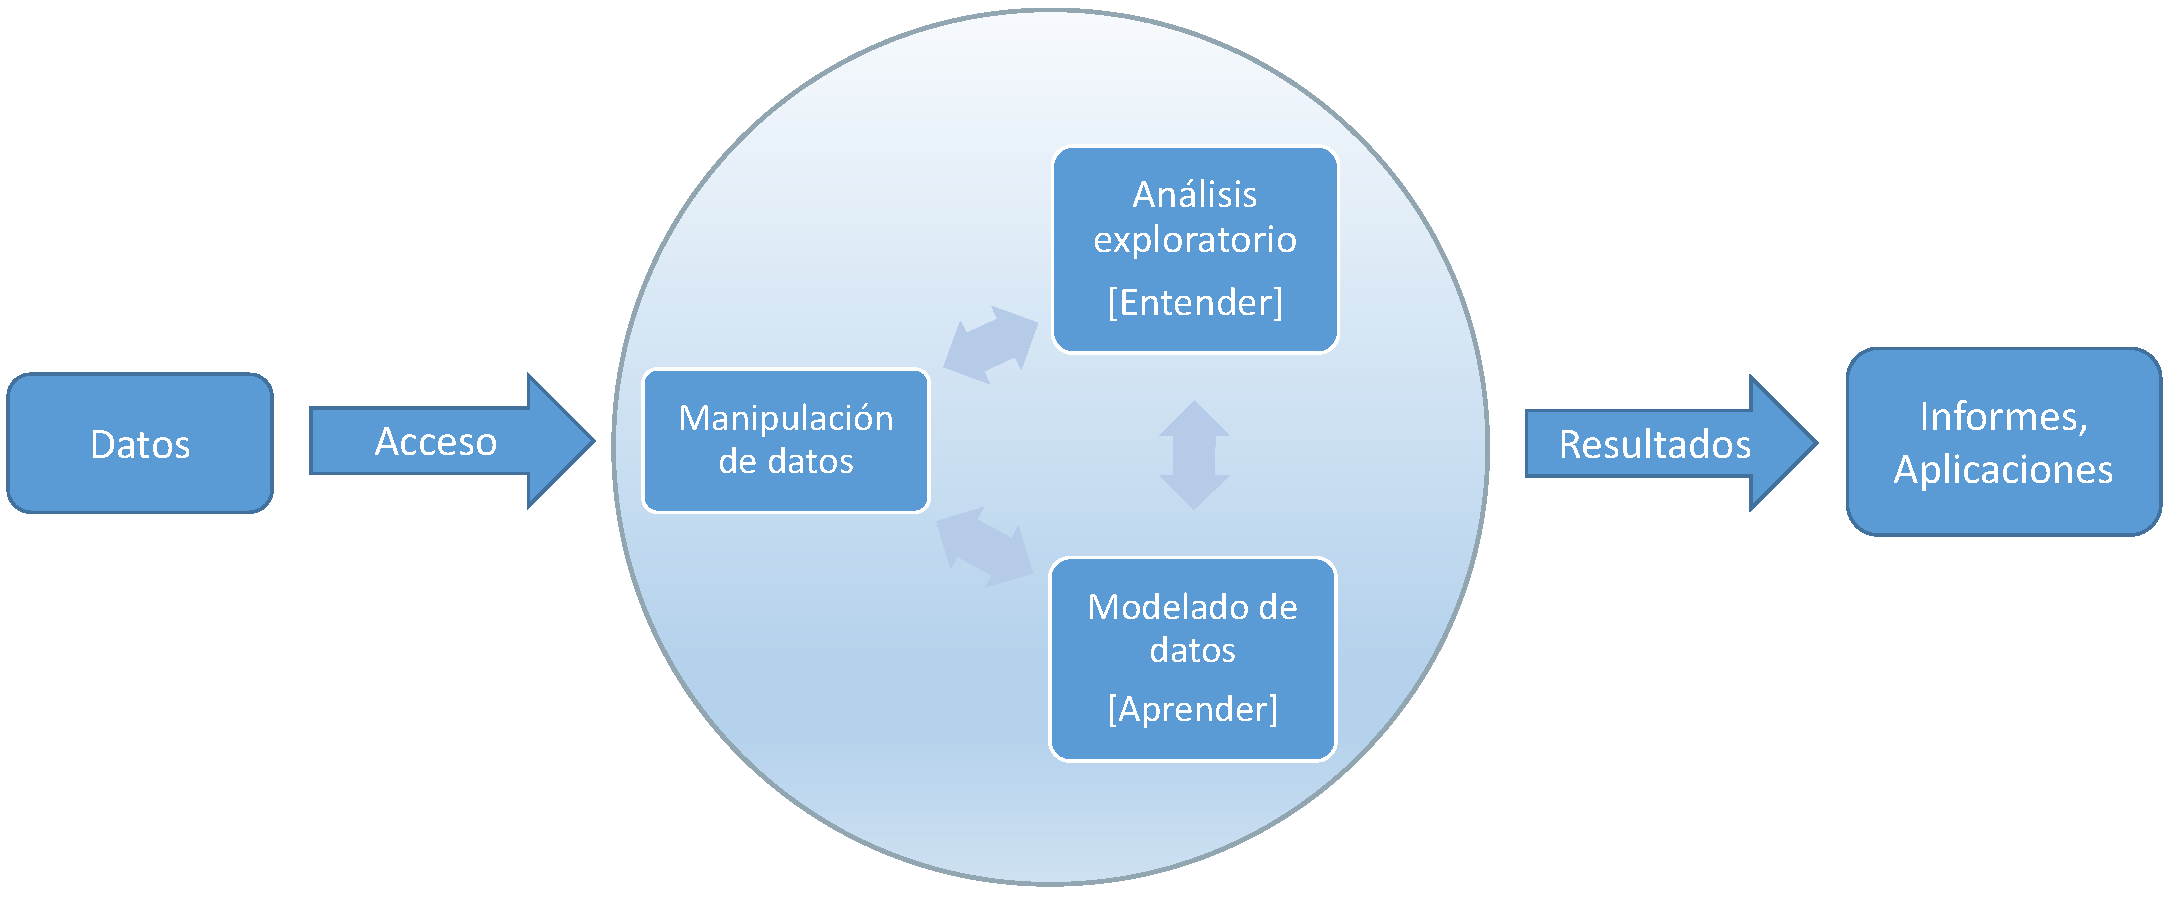
\includegraphics[width=0.8\linewidth]{figuras/esquema2} 

}

\caption{Etapas del proceso}\label{fig:esquema}
\end{figure}

Para una introducción a la programación en R se puede consultar el libro:

Fernández-Casal R., Roca-Pardiñas J., Costa J. y Oviedo-de la Fuente M. (2022). \emph{\href{https://rubenfcasal.github.io/intror}{Introducción al Análisis de Datos con R}} (\href{https://github.com/rubenfcasal/intror}{github}).

Adicionalmente, en este \href{https://rubenfcasal.github.io/post/ayuda-y-recursos-para-el-aprendizaje-de-r}{post} se incluyen enlaces a recursos adicionales, incluyendo libros y cursos, que pueden ser útiles para el aprendizaje de R.

El primer paso es la instalación de R, para ello se recomienda seguir los pasos en este \href{https://rubenfcasal.github.io/post/instalacion-de-r}{post}.

Para el desarrollo de código e informes la recomendación es emplear \emph{RStudio Desktop}, que se puede instalar y configurar siguiendo las indicaciones en este \href{https://rubenfcasal.github.io/post/instalacion-de-rstudio}{post}.
También puede resultar de interés consultar:

\begin{itemize}
\item
  \href{https://posit.co/wp-content/uploads/2022/10/rstudio-ide-1.pdf}{RStudio IDE Cheat Sheet} (menú de RStudio \emph{Help \textgreater{} Cheat Sheets \textgreater{} RStudio IDE Cheat Sheet}).
\item
  \href{https://support.posit.co/hc/en-us/sections/200107586-Using-the-RStudio-IDE}{Using the RStudio IDE}.
\end{itemize}

Sin embargo, en ciertos casos puede ser recomendable ejecutar el código R directamente desde una ventana de comandos (por ejemplo para ejecutar varios programas de forma simultánea en distintos directorios de trabajo o si los requerimientos computacionales son grandes).
En mi caso, cuando trabajo en Windows, acostumbro a emplear el explorador para situarme en el directorio donde quiero ejecutar código y abrir una ventana de comandos, escribiendo \texttt{cmd} en el cuadro superior donde se muestra la ruta.
Posteriormente, como añadí en directorio de instalación de R al \emph{path} (ver \href{https://rubenfcasal.github.io/post/instalacion-de-r/\#rtools}{post}), ejecuto\footnote{También se puede ejecutar un script de R de forma no interactiva ejecutando en el intérprete de comandos del sistema operativo: \texttt{R\ CMD\ BATCH\ {[}opciones{]}\ mi\_script.R\ {[}fichero\_salida{]}} (cambiando \texttt{R} por la ruta completa, e.g.~\texttt{"C:\textbackslash{}Program\ Files\textbackslash{}R\textbackslash{}R-4.2.1\textbackslash{}bin\textbackslash{}R.exe"}, si no se añadió al path. También se puede incluir en un fichero \emph{.bat}, para poder ejecutarlo repetidas veces con mayor facilidad). Ver \href{https://cran.r-project.org/doc/manuals/r-release/R-intro.html\#Invoking-R}{Appendix B Invoking R} de \href{https://cran.r-project.org/doc/manuals/r-release/R-intro.html}{Introduction to R} para información sobre las distintas opciones.} \texttt{R} y finalmente un comando de la forma:

\begin{Shaded}
\begin{Highlighting}[]
\FunctionTok{source}\NormalTok{(}\StringTok{"mi\_script.R"}\NormalTok{, }\AttributeTok{echo =} \ConstantTok{TRUE}\NormalTok{, }\AttributeTok{encoding =} \StringTok{"UTF{-}8"}\NormalTok{) }\CommentTok{\# UTF{-}8 importante en R \textless{} 4.2}
\end{Highlighting}
\end{Shaded}

\hypertarget{organizacion}{%
\section{Organización}\label{organizacion}}

Para la organización de archivos (datos, código, informes\ldots) lo recomendable es emplear un directorio con la estructura adecuada.

Dependiendo del objetivo puede interesar emplear un proyecto de RStudio (menú \emph{File \textgreater{} New project\ldots{}}).
En mi caso empleo esta opción para paquetes, libros en bookdown, webs con blogdown y aplicaciones shiny.
En otros casos empleo una carpeta que puede tener subdirectorios (si el proyecto es más grande) para distintos tipos de archivos o para distintas tareas (con el objetivo de facilitar la búsqueda).
Por ejemplo: \emph{datos}, \emph{informes}, \emph{resultados\_2023}\ldots{}

Mi recomendación es emplear nombres de archivos y carpetas en minúscula (o con la primera letra en mayúsculas), sin espacios (por ejemplo empleando \texttt{\_} para separar palabras o iniciales) y sin caracteres especiales (ASCII, sin acentos\ldots).
Los nombres deberían ser lo más descriptivos posibles (en el sentido de evitar confusión).
Pueden incluirse descripciones más completas en el código, en ficheros de texto (e.g.~\emph{Descripcion\_archivos.txt}), o incluso en hojas de cálculo.
Yo además acostumbro a incluir archivos del tipo \emph{Notas.txt} (con recordatorios, decisiones\ldots) o \emph{Pendente.txt} (con próximos pasos, mejoras o verificaciones pendientes\ldots).

Además, nos puede interesar establecer opciones de R específicas para el proyecto (por ejemplo opciones de configuración de memoria, de paquetes o variables de entorno, incluyendo claves privadas), de forma que se establezcan automáticamente al iniciar R o RStudio.
Para más detalles ver la ayuda de \texttt{?Startup}, el apéndice \href{https://cran.r-project.org/doc/manuals/r-release/R-intro.html\#Invoking-R}{Invoking R} o el post de RStudio
\href{https://support.posit.co/hc/en-us/articles/360047157094-Managing-R-with-Rprofile-Renviron-Rprofile-site-Renviron-site-rsession-conf-and-repos-conf}{Managing R with .Rprofile, .Renviron, Rprofile.site, Renviron.site, rsession.conf, and repos.conf}

Para desarrollar código y proyectos de forma colaborativa, la recomendación es emplear un sistema de control de versiones.
Se puede configurar RStudio para emplear Git (ver el libro \href{https://happygitwithr.com/index.html}{Happy Git and GitHub for the useR} o la sección \href{https://r-pkgs.org/software-development-practices.html\#sec-sw-dev-practices-git-github}{Git and GitHub}), sin embargo yo prefiero emplear \href{https://desktop.github.com/}{GitHub Desktop}.

\hypertarget{codigo}{%
\subsection{Código e informes}\label{codigo}}

Mi recomendación a la hora de escribir código es seguir un \textbf{proceso iterativo}.
Se comienza realizando pruebas y al finalizar cada etapa se trata de reorganizar el código (adaptándolo al estilo de programación elegido, lo que incluiría añadir comentarios y secciones) de forma que sea más cómodo continuar trabajando en siguientes etapas (y si es posible que resulte más fácil de adaptar para otros casos).

En el caso de informes el proceso sería similar, empleando como punto de partida un fichero de código en formato \href{https://yihui.org/knitr/demo/stitch/\#spin-comment-out-texts}{spin} (ver Sección \ref{spin}), en el que el texto RMarkdown se incluye como un comentario de código empleando \texttt{\#\textquotesingle{}}.
Por ejemplo:

\begin{verbatim}
#' # Sección
#'
#' ## Subsección
#'
#' Texto rmarkdown...
\end{verbatim}

En primer lugar me preocupo de escribir un código funcional y, además de ir añadiendo comentarios de la forma habitual, voy añadiendo secciones y texto rmarkdown en formato spin.
Finalmente, cuando tengo una primera versión del código (que puedo ir previsualizando; en RStudio basta con pulsar\footnote{Para mostrar las combinaciones de teclas en RStudio podemos emplear el menú \emph{Tools \textgreater{} Keyboard Shortcuts Help}.} \emph{Ctrl + Shift + K}, el icono correspondiente en la barra superior, o seleccionar \emph{File \textgreater{} Compile Report\ldots{}}), lo transformo a formato \emph{.Rmd} con un comando de la forma:

\begin{Shaded}
\begin{Highlighting}[]
\NormalTok{knitr}\SpecialCharTok{::}\FunctionTok{spin}\NormalTok{(}\StringTok{"Informe.R"}\NormalTok{, }\AttributeTok{knit =} \ConstantTok{FALSE}\NormalTok{)}
\end{Highlighting}
\end{Shaded}

donde termino de redactar (\texttt{knitr::purl("Informe.Rmd",\ documentation\ =\ 2)} genera un nuevo fichero \emph{Informe.R} donde resulta más cómodo modificar o desarrollar código).

Se recomienda \textbf{elegir un estilo que sea consistente y seguirlo por completo} en todo el proyecto.
Lo principal sería el operador de asignación, el espaciado y el estilo de nombres (de objetos, variables o ficheros):

\begin{itemize}
\item
  \texttt{estilo.clasico}: es el estilo del paquete base de R. Muchos programadores no lo recomiendan (principalmente porque este separador no se admite en otros lenguajes y porque puede dar lugar a confusión con métodos S3, ver Sección \ref{oop}).
\item
  \texttt{estilo\_serpiente} (o \texttt{Estilo\_serpiente}): es el estilo de la colección de paquetes \href{https://tidyverse.tidyverse.org}{\texttt{tidyverse}}.
\item
  \texttt{EstiloCamello} (o \texttt{estiloCamello}): es el estilo (casi obligatorio) para las clases \href{https://r6.r-lib.org}{\texttt{R6}} (ver Sección \ref{oop}). El paquete \href{https://shiny.rstudio.com/}{\texttt{shiny}} emplea la variante que comienza por minúsculas.
\end{itemize}

\textbf{Recomiendo emplear \texttt{\textless{}-}} como operador de asignación y escribir todos los \textbf{nombres en minúsculas}.
Yo tengo tendencia a emplear el \texttt{estilo.clasico}, sobre todo si el código no depende de paquetes tidyverse (en ese caso suelo emplear \texttt{estilo\_serpiente}).
También influye el estilo de nombres empleado por la fuente de datos o el requerido en los resultados.

El estilo también debe especificar el sangrado, el espaciado, etc.
Por ejemplo:

\begin{itemize}
\item
  \href{https://style.tidyverse.org}{Tidyverse style guide}
\item
  \href{https://google.github.io/styleguide/Rguide.html}{Google's R Style Guide}
\end{itemize}

Para facilitar la legibilidad \textbf{es muy recomendable incluir un espacio} entre los elementos del comando.
En RStudio se puede seleccionar un trozo de (una línea de) código y pulsar \emph{Ctrl + Shift + A} para formatearlo.
También podemos emplear el paquete \href{https://github.com/r-lib/styler}{\texttt{styler}} para formatear el código.
Por ejemplo, en RStudio podemos emplear \emph{Addins \textgreater{} Styler \textgreater{} Style active file}.

Además se recomienda \textbf{crear secciones y documentar el código adecuadamente}.
En RStudio se puede crear una sección pulsando \emph{Ctrl + Shift + R} o añadiendo al menos 4 guiones (\texttt{-}, también \texttt{=} o \texttt{\#}) después de un comentario.
Por ejemplo:

\begin{Shaded}
\begin{Highlighting}[]
\CommentTok{\# Sección {-}{-}{-}{-}}
\DocumentationTok{\#\# Subsección {-}{-}{-}{-}}
\end{Highlighting}
\end{Shaded}

El orden de las secciones y subsecciones es importante.
Al principio del código debería ir:

\begin{enumerate}
\def\labelenumi{\arabic{enumi}.}
\tightlist
\item
  Los parámetros o variables globales.
\item
  La carga de paquetes (únicamente los mínimos requeridos).
\item
  La carga de código externo.
\item
  La carga de archivos de datos (o al principio de la sección donde se emplean, si son datos auxiliares).
\end{enumerate}

\textbf{No se recomienda} emplear rutas absolutas en el código, del tipo:

\begin{Shaded}
\begin{Highlighting}[]
\FunctionTok{setwd}\NormalTok{(}\StringTok{"C:/Documentos/Proyectos/Proyecto\_X"}\NormalTok{)}
\FunctionTok{load}\NormalTok{(}\StringTok{"C:/Documentos/Proyectos/Proyecto\_X/datos\_x.RData"}\NormalTok{)}
\FunctionTok{source}\NormalTok{(}\StringTok{"C:/Documentos/Proyectos/R/Herramientas.R"}\NormalTok{)}
\end{Highlighting}
\end{Shaded}

Como punto de partida el directorio de trabajo debería ser la carpeta del proyecto.
Esto ya ocurre por defecto si empleamos proyectos de RStudio o si iniciamos RStudio abriendo un archivo de código en esta carpeta.
En general, la recomendación es asumir que el directorio de trabajo es aquel en el que se encuentra el archivo de código (lo que también ocurre por defecto al compilar un documento RMarkdown).
Si no es el caso se puede emplear el menú \emph{Sesion \textgreater{} Set Working Directory \textgreater{} To Source File Location}.

Para establecer la ruta a archivos o directorios \textbf{se recomienda emplear rutas relativas} (usando \emph{../} para acceder a la carpeta anterior; \emph{./} sería el actual directorio de trabajo).
Por ejemplo:

\begin{Shaded}
\begin{Highlighting}[]
\FunctionTok{load}\NormalTok{(}\StringTok{"datos/datos\_x.RData"}\NormalTok{)}
\FunctionTok{source}\NormalTok{(}\StringTok{"../R/Herramientas.R"}\NormalTok{)}
\NormalTok{fecha\_txt }\OtherTok{\textless{}{-}} \FunctionTok{as.character}\NormalTok{(}\FunctionTok{Sys.Date}\NormalTok{() }\SpecialCharTok{{-}} \DecValTok{1}\NormalTok{, }\AttributeTok{format =} \StringTok{"\%m\_\%d"}\NormalTok{) }\CommentTok{\# Por ejemplo...}
\NormalTok{rmarkdown}\SpecialCharTok{::}\FunctionTok{render}\NormalTok{(}\StringTok{"informe.Rmd"}\NormalTok{, }\AttributeTok{params =} \FunctionTok{list}\NormalTok{(}\AttributeTok{fecha\_txt =}\NormalTok{ fecha\_txt),}
                  \AttributeTok{output\_file =} \FunctionTok{paste0}\NormalTok{(}\StringTok{\textquotesingle{}informes/informe\_\textquotesingle{}}\NormalTok{, fecha\_txt, }\StringTok{\textquotesingle{}.html\textquotesingle{}}\NormalTok{), }
                  \AttributeTok{envir =} \FunctionTok{new.env}\NormalTok{(), }\AttributeTok{encoding =} \StringTok{"UTF{-}8"}\NormalTok{)}
\end{Highlighting}
\end{Shaded}

La mejor forma de organizar funciones es desarrollar un paquete, como se comenta más adelante en la Sección \ref{desarrollo}.

\hypertarget{datos}{%
\subsection{Datos}\label{datos}}

La recomendación es emplear ficheros de datos con el formato por defecto de R (datos binarios comprimidos), con extensión \emph{.RData}.
Hay que tener en cuenta que lo esperable es que el archivo contenga un conjunto de datos con el mismo nombre, aunque podría no ser el caso e incluso contener varios objetos.

Uno de los problemas con los ficheros \emph{.RData} es que, al cargarlos con \href{https://rdrr.io/r/base/load.html}{\texttt{load()}} de la forma habitual, se añaden al entorno de trabajo los objetos que contienen con los nombres con que se almacenaron (y si ya existe alguno con ese nombre lo sobreescribe)
Para almacenar un único objeto de forma que se pueda cargar posteriormente especificando el nombre, se pueden emplear las funciones \href{https://rdrr.io/r/base/readRDS.html}{\texttt{saveRDS()}} y \href{https://rdrr.io/r/base/readRDS.html}{\texttt{readRDS()}}.

Sin embargo, lo habitual es que inicialmente los datos procedan de una fuente externa.
Se pueden importar datos externos en casi cualquier formato a R (aunque puede requerir instalar paquetes adicionales).
Mi recomendación es separar los análisis de la importación de los datos.
Crear un fichero de código específicamente para importar los datos\footnote{Con algunos tipos de datos, se puede emplear los submenús de RStudio \emph{File \textgreater{} Import Dataset} para seleccionar los ajustes, previsualizando el resultado, y generar el código para importarlos.}, hacer el (pre)procesado y guardarlos en formato \emph{.RData}.
Yo habitualmente empleo el mismo nombre para el archivo de código y el archivo de datos que se genera (e.g.~\emph{datos.R} contiene el código necesario para generar \emph{datos.RData}; no suelo renombrar el fichero fuente de datos externo, aunque se aleje mucho del estilo elegido).
Asociado a un mismo conjunto de datos puede haber distintos archivos de código para realizar distintos análisis (el nombre de esos archivos debería dar una pista del análisis que realizan).

En muchas ocasiones, para modificar los nombres de las variables o los niveles de un factor, suelo recurrir a la función \href{https://rdrr.io/r/base/dput.html}{\texttt{dput()}} para escribirlos en modo texto (e.g.~\texttt{dput(tolower(names(datos)))} o \texttt{dput(levels(datos\$factor))}) y posteriormente modificarlos a mano.

Yo recomiendo añadir un atributo \texttt{variable.labels} que contenga un vector de etiquetas de las variables y empleando como nombres de las componentes las propias variables:

\begin{Shaded}
\begin{Highlighting}[]
\FunctionTok{data}\NormalTok{(cars)}
\CommentTok{\# dput(names(cars))}
\NormalTok{var.lab }\OtherTok{\textless{}{-}} \FunctionTok{c}\NormalTok{(}\AttributeTok{speed =} \StringTok{"Speed (mph)"}\NormalTok{, }\AttributeTok{dist =} \StringTok{"Stopping distance (ft)"}\NormalTok{)}
\FunctionTok{attr}\NormalTok{(cars, }\StringTok{"variable.labels"}\NormalTok{) }\OtherTok{\textless{}{-}}\NormalTok{ var.lab}
\FunctionTok{str}\NormalTok{(cars)}
\end{Highlighting}
\end{Shaded}

\begin{verbatim}
## 'data.frame':    50 obs. of  2 variables:
##  $ speed: num  4 4 7 7 8 9 10 10 10 11 ...
##  $ dist : num  2 10 4 22 16 10 18 26 34 17 ...
##  - attr(*, "variable.labels")= Named chr [1:2] "Speed (mph)" "Stopping distance (ft)"
##   ..- attr(*, "names")= chr [1:2] "speed" "dist"
\end{verbatim}

\begin{Shaded}
\begin{Highlighting}[]
\CommentTok{\# View(cars)}
\CommentTok{\# with(cars, plot(speed, dist, xlab = var.lab["speed"], }
\CommentTok{\#                 ylab = var.lab["dist"]))}
\end{Highlighting}
\end{Shaded}

Para leer ficheros de Excel acostumbro a utilizar los paquetes \href{https://cran.r-project.org/web/packages/openxlsx/index.html}{\texttt{openxlsx}} (solo para archivos con extensión \emph{.xlsx}) o \href{https://readxl.tidyverse.org}{\texttt{readxl}} (colección \href{https://www.tidyverse.org/}{\texttt{tidyverse}}; Sección \ref{tidyverse}).
En estos casos además se puede añadir una nueva hoja de cálculo con los nombres de las variables junto con su etiqueta, que se puede cargar y emplear durante el preprocesado.
Adicionalmente esta tabla puede incluir una columna con los nuevos nombres (yo recomiendo no modificar los antiguos en este fichero), otra con un filtro para seleccionar variables (o el orden después del procesado) e incluso una columna con anotaciones o observaciones.
Ver \href{ejemplos/top500/top500.R}{top500.R} en \href{https://github.com/rubenfcasal/book_notasr/tree/main/ejemplos}{ejemplos}.

\hypertarget{part-el-entorno-estaduxedstico-r}{%
\part{El entorno estadístico R}\label{part-el-entorno-estaduxedstico-r}}

\hypertarget{r}{%
\chapter{El lenguaje R}\label{r}}

Cualquier análisis de R requiere programación, aunque normalmente se puede llevar a cabo sin conocimientos profundos del lenguaje (\emph{useR}).
Sin embargo, para desarrollar nuevas herramientas de forma efectiva (\emph{programeR}) es necesario tener una idea del funcionamiento interno de R.
La referencia recomendada para usuarios de R que deseen mejorar sus conocimientos de programación y comprensión del lenguaje es:

Wickham, Hadley (2019). \emph{\href{https://adv-r.hadley.nz/}{Advanced R, 2ª edición}}, \href{https://www.amazon.com/dp/0815384572}{Chapman \& Hall}, \href{http://adv-r.had.co.nz/}{1ª edición}.

También puede ser de utilidad el manual \href{https://cran.r-project.org/doc/manuals/R-lang.html}{R Language Definition}
para consultas adicionales\footnote{Los manuales oficiales también están disponibles en formato bookdown en este \href{https://colinfay.me/r-manuals}{post}.}.

\hypertarget{paquetes}{%
\section{Paquetes}\label{paquetes}}

Al instalar R se instalan los denominados \textbf{paquetes base} y (por defecto) los \textbf{paquetes recomendados} por los desarrolladores de R (el \emph{R Core Team}).
Podemos acceder a la lista de paquetes instalados:

\begin{Shaded}
\begin{Highlighting}[]
\NormalTok{pkgs }\OtherTok{\textless{}{-}} \FunctionTok{installed.packages}\NormalTok{()}
\FunctionTok{names}\NormalTok{(}\FunctionTok{which}\NormalTok{(pkgs[ ,}\StringTok{"Priority"}\NormalTok{] }\SpecialCharTok{==} \StringTok{"base"}\NormalTok{))}
\end{Highlighting}
\end{Shaded}

\begin{verbatim}
##  [1] "base"      "compiler"  "datasets"  "graphics"  "grDevices" "grid"     
##  [7] "methods"   "parallel"  "splines"   "stats"     "stats4"    "tcltk"    
## [13] "tools"     "utils"
\end{verbatim}

\begin{Shaded}
\begin{Highlighting}[]
\FunctionTok{names}\NormalTok{(}\FunctionTok{which}\NormalTok{(pkgs[ ,}\StringTok{"Priority"}\NormalTok{] }\SpecialCharTok{==} \StringTok{"recommended"}\NormalTok{))}
\end{Highlighting}
\end{Shaded}

\begin{verbatim}
##  [1] "boot"       "class"      "cluster"    "codetools"  "foreign"   
##  [6] "KernSmooth" "lattice"    "MASS"       "Matrix"     "mgcv"      
## [11] "nlme"       "nnet"       "rpart"      "spatial"    "survival"
\end{verbatim}

Para instalar paquetes adicionales se puede emplear \texttt{install.packages()} (actualmente, 2023-04-01, están disponibles 19217 en \href{https://cran.r-project.org/web/packages/available_packages_by_date.html}{CRAN}, incluso para interactuar con ChatGPT como \href{https://michelnivard.github.io/gptstudio}{\texttt{gptstudio}}).
Por ejemplo:

\begin{Shaded}
\begin{Highlighting}[]
\NormalTok{pkgs }\OtherTok{\textless{}{-}} \FunctionTok{c}\NormalTok{(}\StringTok{"Rcmdr"}\NormalTok{, }\StringTok{"caret"}\NormalTok{, }\StringTok{"tidymodels"}\NormalTok{, }\StringTok{"tidyverse"}\NormalTok{, }\StringTok{"remotes"}\NormalTok{, }\StringTok{"devtools"}\NormalTok{,}
          \StringTok{"sf"}\NormalTok{, }\StringTok{"gstat"}\NormalTok{, }\StringTok{"geoR"}\NormalTok{, }\StringTok{"quadprog"}\NormalTok{, }\StringTok{"DEoptim"}\NormalTok{, }\StringTok{"spam"}\NormalTok{, }\StringTok{"openxlsx"}\NormalTok{,}
            \StringTok{"bookdown"}\NormalTok{, }\StringTok{"blogdown"}\NormalTok{, }\StringTok{"pkgdown"}\NormalTok{)}
\FunctionTok{install.packages}\NormalTok{(}\FunctionTok{setdiff}\NormalTok{(pkgs, }\FunctionTok{installed.packages}\NormalTok{()[,}\StringTok{"Package"}\NormalTok{]), }\AttributeTok{dependencies =} \ConstantTok{TRUE}\NormalTok{)}
\end{Highlighting}
\end{Shaded}

En Windows (y en MacOS) esta función instala por defecto paquetes compilados (\texttt{type\ =\ "binary"}, que dependen del sistema operativo y de la versión R) disponibles en CRAN.
Aunque podría instalar paquetes disponibles en otros repositorios.
Por ejemplo:

\begin{Shaded}
\begin{Highlighting}[]
\NormalTok{url }\OtherTok{\textless{}{-}} \StringTok{"https://github.com/rubenfcasal/simres/releases/download/v0.1/simres\_0.1.3.zip"}
\FunctionTok{install.packages}\NormalTok{(url, }\AttributeTok{repos =} \ConstantTok{NULL}\NormalTok{)}
\end{Highlighting}
\end{Shaded}

También se pueden instalar paquetes directamente a partir del código fuente con \texttt{type\ =\ "source"} (por defecto en Linux), pero en ciertos casos es necesario tener instaladas herramientas adicionales (por ejemplo \href{https://cran.r-project.org/bin/windows/Rtools}{Rtools} en Windows si el paquete contiene código en C, C++ o Fortran).
Esto permitiría incluso instalar paquetes retirados de CRAN (e.g.~actualmente \href{https://CRAN.R-project.org/package=kedd}{\texttt{kedd}}), ya que siempre se mantiene el código (en un archivo comprimido de la forma \texttt{paquete\_x.y.z.tar.gz}).

Si se quieren instalar paquetes de repositorios distintos de CRAN (GitHub, GitLab, Bitbucket\ldots), puede ser recomendable instalar \href{https://remotes.r-lib.org/}{\texttt{remotes}}.
Por ejemplo:

\begin{Shaded}
\begin{Highlighting}[]
\NormalTok{remotes}\SpecialCharTok{::}\FunctionTok{install\_github}\NormalTok{(}\StringTok{"rubenfcasal/simres"}\NormalTok{, }\AttributeTok{INSTALL\_opts =} \StringTok{"{-}{-}with{-}keep.source"}\NormalTok{)}
\end{Highlighting}
\end{Shaded}

Además puede ser de utilidad mantener los comentarios originales del paquete para entender mejor el código (por ejemplo si se quiere modificar).

Otras funciones que pueden ser de interés son: \texttt{remove.packages()}, \texttt{update.packages()} y \texttt{available.packages()}.

Al iniciar el programa \texttt{R} se cargan por defecto en memoria los principales paquetes base, añadiéndolos a la ruta de búsqueda (a continuación del entorno de trabajo \texttt{.GlobalEnv} y siempre terminando con en el paquete \texttt{base}, el primero que se carga):

\begin{Shaded}
\begin{Highlighting}[]
\FunctionTok{search}\NormalTok{()}
\end{Highlighting}
\end{Shaded}

\begin{verbatim}
##  [1] ".GlobalEnv"        "package:dbplyr"    "package:forcats"  
##  [4] "package:stringr"   "package:dplyr"     "package:purrr"    
##  [7] "package:readr"     "package:tidyr"     "package:tibble"   
## [10] "package:ggplot2"   "package:tidyverse" "package:magrittr" 
## [13] "package:stats"     "package:graphics"  "package:grDevices"
## [16] "package:utils"     "package:datasets"  "package:methods"  
## [19] "Autoloads"         "package:base"
\end{verbatim}

Concretamente se añade a la ruta de búsqueda un entorno que contiene el conjunto de objetos exportables del paquete, definido en el denominado \textbf{\emph{namespace}} del paquete.
Esta ruta determina los objetos visibles en el entorno global y el orden en se buscan (para más detalles ver \href{https://adv-r.hadley.nz/environments.html\#env-basics}{7.2 Environment basics} y \href{https://adv-r.hadley.nz/environments.html\#special-environments}{7.4 Special environments} de \href{https://adv-r.hadley.nz/index.html}{Advanced R}).

Podemos cargar paquetes adicionales (previamente instalados) con \texttt{library()} o \texttt{require()}, por ejemplo:

\begin{Shaded}
\begin{Highlighting}[]
\ControlFlowTok{if}\NormalTok{ (}\SpecialCharTok{!}\FunctionTok{require}\NormalTok{(knitr)) \{}
  \FunctionTok{install.packages}\NormalTok{(}\StringTok{"knitr"}\NormalTok{)}
  \FunctionTok{library}\NormalTok{(knitr)}
\NormalTok{\}}
\FunctionTok{spin}\NormalTok{(}\StringTok{"01{-}Introduccion.R"}\NormalTok{, }\AttributeTok{knit =} \ConstantTok{FALSE}\NormalTok{)}
\end{Highlighting}
\end{Shaded}

Aunque \textbf{no se recomienda que el código instale automáticamente paquetes} (en general que haga cambios en la configuración del equipo en el que se ejecuta).

Al cargar un paquete se añade por defecto en la segunda posición de la ruta de búsqueda (justo después del entorno global, desplazando al resto).
También se podrían añadir otros objetos, por ejemplo data.frames, con la función \texttt{attach()} pero \textbf{no se recomienda} (se puede utilizar \texttt{with()} como alternativa).

Hay que tener cuidado con las versiones instaladas de los paquetes:

\begin{Shaded}
\begin{Highlighting}[]
\FunctionTok{packageVersion}\NormalTok{(}\StringTok{"dplyr"}\NormalTok{)}
\end{Highlighting}
\end{Shaded}

\begin{verbatim}
## [1] '1.0.10'
\end{verbatim}

y con sus dependencias (los paquetes tienen su propia ruta de búsqueda, determinada por el \emph{namespace} del paquete).
Al actualizar o instalar nuevos paquetes pueden aparecer problemas al ejecutar código antiguo (a veces al trabajar en nuevos proyectos acabamos haciendo que los antiguos dejen de funcionar).

Se puede instalar versiones específicas de un paquete con \href{https://remotes.r-lib.org/reference/install_version.html}{\texttt{remotes::install\_version()}}:

\begin{Shaded}
\begin{Highlighting}[]
\NormalTok{remotes}\SpecialCharTok{::}\FunctionTok{install\_version}\NormalTok{(}\StringTok{"dplyr"}\NormalTok{, }\AttributeTok{version =} \StringTok{"1.11"}\NormalTok{) }\CommentTok{\# repos = "https://ftp.cixug.es/CRAN")}
\end{Highlighting}
\end{Shaded}

Para asegurarse que el código de un proyecto se pueda ejecutar a lo largo del tiempo se puede emplear el paquete \href{https://rstudio.github.io/renv/}{\texttt{renv}} (se puede configurar automáticamente al crear un proyecto de RStudio).
Este paquete permite registrar las versiones exactas de los paquetes de los que depende un proyecto y volver a instalarlas (incluso en otro equipo) si es necesario. Para más detalles ver la viñeta \href{https://rstudio.github.io/renv/articles/renv.html}{Introduction to renv}.

Sin embargo de esta forma aún dependemos del sistema operativo que deberíamos configurar adecuadamente.
La recomendación para que un proyecto en R (por ejemplo una aplicación shiny) se pueda ejecutar en cualquier equipo, es emplear un \href{https://es.wikipedia.org/wiki/Docker_(software)}{contenedor docker}.
Para más detalles ver \href{https://docs.docker.com/get-started/overview/}{Docker overview} y \href{https://rocker-project.org/}{The Rocker Project}.
Ver \href{ejemplos/covid19/prediccion_cooperativa/vii_xornadasr.html}{ejemplos/covid19/prediccion\_cooperativa}.

\hypertarget{funciones}{%
\section{Funciones}\label{funciones}}

\begin{quote}
``Everything that happens in R is the result of a function call''.

--- John M. Chambers
\end{quote}

Como es bien conocido, en R se pueden asignar los argumentos de una función por posición o por nombre (del correspondiente parámetro en la definición de la función, denominado \emph{argumento formal en R}).
En general, la recomendación es asignar los argumentos por nombre:

\texttt{funcion(parametro1\ =\ argumento1,\ parametro2\ =\ argumento2,\ ...)}

De esta forma no importa el orden de los parámetros y, por ejemplo, evitaremos problemas si en el futuro hay cambios en la definición de la función.
Los parámetros pueden tener valores por defecto y solo sería necesario especificarlos para asignarles un valor distinto.

Podemos llamar a una función de un paquete sin necesidad de cargarlo (añadirlo a la ruta de búsqueda) empleando \texttt{paquete::funcion}.
Esto es especialmente recomendable al desarrollar nuevas funciones (es un requisito para subir paquetes a CRAN), ya que de esta forma se evitan conflictos entre funciones con el mismo nombre en paquetes distintos.
Por ejemplo:

\begin{Shaded}
\begin{Highlighting}[]
\ControlFlowTok{if}\NormalTok{ (}\SpecialCharTok{!}\FunctionTok{requireNamespace}\NormalTok{(}\StringTok{"knitr"}\NormalTok{)) }\FunctionTok{stop}\NormalTok{(}\StringTok{"\textquotesingle{}knitr\textquotesingle{} package required"}\NormalTok{)}
\NormalTok{knitr}\SpecialCharTok{::}\FunctionTok{spin}\NormalTok{(}\StringTok{"01{-}Introduccion.R"}\NormalTok{, }\AttributeTok{knit =} \ConstantTok{FALSE}\NormalTok{)}
\end{Highlighting}
\end{Shaded}

Hay que tener en cuenta que R emplea \href{https://adv-r.hadley.nz/functions.html\#lazy-evaluation}{Lazy evaluation}, los argumentos no se evalúan hasta que se necesitan (lo cual puede producir mensajes de error inesperados, pero también permite añadir funcionalidades adicionales empleando la denominada \href{http://adv-r.had.co.nz/Computing-on-the-language.html}{evaluación no estándar} o \href{https://adv-r.hadley.nz/metaprogramming.html}{metaprogramación}).

R es un lenguaje interpretado y podemos evaluar expresiones empleando código.
Por ejemplo, podemos reproducir el proceso de introducir un comando en la consola con las funciones \texttt{eval()} y \texttt{parse()} (aunque esta forma de proceder no es la más eficiente):

\begin{Shaded}
\begin{Highlighting}[]
\FunctionTok{eval}\NormalTok{(}\FunctionTok{parse}\NormalTok{(}\AttributeTok{text =} \StringTok{"1:10"}\NormalTok{))}
\end{Highlighting}
\end{Shaded}

\begin{verbatim}
##  [1]  1  2  3  4  5  6  7  8  9 10
\end{verbatim}

\begin{Shaded}
\begin{Highlighting}[]
\NormalTok{distr }\OtherTok{\textless{}{-}} \StringTok{"norm"}  \CommentTok{\# "unif", "exp", "t"}
\NormalTok{ddistr }\OtherTok{\textless{}{-}} \FunctionTok{eval}\NormalTok{(}\FunctionTok{parse}\NormalTok{(}\AttributeTok{text =} \FunctionTok{paste0}\NormalTok{(}\StringTok{"d"}\NormalTok{, distr)))}
\CommentTok{\# str(ddistr)}
\CommentTok{\# curve(ddistr(x, 0, 0.5), {-}3, 3)}
\end{Highlighting}
\end{Shaded}

Para llamar a una función especificando los parámetros de forma dinámica (empleando una lista) podemos emplear \texttt{do.call()}.
Por ejemplo:

\begin{Shaded}
\begin{Highlighting}[]
\CommentTok{\# Listar ficheros csv }
\NormalTok{files.csv }\OtherTok{\textless{}{-}} \FunctionTok{dir}\NormalTok{(}\AttributeTok{path =} \StringTok{"datos"}\NormalTok{, }\AttributeTok{pattern =} \StringTok{"*.csv"}\NormalTok{, }\AttributeTok{full.names =} \ConstantTok{TRUE}\NormalTok{)}
\CommentTok{\# Leer datos a una lista}
\CommentTok{\# (suponemos variante local con ; para separar valores)}
\NormalTok{data.list }\OtherTok{\textless{}{-}} \FunctionTok{lapply}\NormalTok{(files.csv, read.csv2)}
\CommentTok{\# Combinar }
\NormalTok{datos }\OtherTok{\textless{}{-}} \FunctionTok{do.call}\NormalTok{(}\StringTok{\textquotesingle{}rbind\textquotesingle{}}\NormalTok{, data.list)}
\end{Highlighting}
\end{Shaded}

R dispone además de otras herramientas que permiten la programación dinámica.
Por ejemplo \href{https://rdrr.io/r/stats/delete.response.html}{\texttt{reformulate()}} permite construir formulas para ajuste de modelos o análisis descriptivos.

Hay que tener en cuenta que las funciones tienen su propio entorno y su propia ruta de búsqueda, determinada por el entorno donde se crearon (el \emph{namespace} en el caso de las funciones de un paquete).
Esto es lo que se conoce como \href{https://adv-r.hadley.nz/functions.html\#lexical-scoping}{Lexical scoping}.

\begin{Shaded}
\begin{Highlighting}[]
\NormalTok{x }\OtherTok{\textless{}{-}} \DecValTok{1}
\NormalTok{addx }\OtherTok{\textless{}{-}} \ControlFlowTok{function}\NormalTok{(y) \{}
\NormalTok{  x }\SpecialCharTok{+}\NormalTok{ y}
\NormalTok{\}}
\FunctionTok{addx}\NormalTok{(}\DecValTok{10}\NormalTok{)}
\end{Highlighting}
\end{Shaded}

\begin{verbatim}
## [1] 11
\end{verbatim}

\begin{Shaded}
\begin{Highlighting}[]
\NormalTok{addx10 }\OtherTok{\textless{}{-}} \ControlFlowTok{function}\NormalTok{() \{}
\NormalTok{  x }\OtherTok{\textless{}{-}} \DecValTok{10}   \CommentTok{\# x \textless{}\textless{}{-} 10   \# assign("x", 10, envir = .GlobalEnv)}
  \FunctionTok{addx}\NormalTok{(x)}
\NormalTok{\}}
\FunctionTok{addx10}\NormalTok{()}
\end{Highlighting}
\end{Shaded}

\begin{verbatim}
## [1] 11
\end{verbatim}

\begin{Shaded}
\begin{Highlighting}[]
\NormalTok{x}
\end{Highlighting}
\end{Shaded}

\begin{verbatim}
## [1] 1
\end{verbatim}

\hypertarget{oop}{%
\section{Programación orientada a objetos (funciones genéricas)}\label{oop}}

\begin{quote}
``Everything that exists in R is an object''.

--- John M. Chambers
\end{quote}

R implementa programación orientada a objetos (OOP).
Por ejemplo, es bien conocido que algunas funciones (entre ellas \texttt{print()}, \texttt{plot()} o \texttt{summary()}) se comportan de manera diferente dependiendo de la clase (el tipo de objeto) de sus argumentos, son las denominadas \emph{funciones genéricas}.

Realmente R dispone de varios sistemas de OOP, entre ellos podríamos destacar (ver capítulos en \href{https://adv-r.hadley.nz/oo.html}{Object-oriented programming} de \href{https://adv-r.hadley.nz}{Advanced R}):

\begin{itemize}
\item
  \href{https://adv-r.hadley.nz/s3.html}{S3}: Es un sistema muy simple, las clases no tienen una definición formal (no se verifica su consistencia). Es el empleado en el paquete \texttt{base} de R y en la mayoría de paquetes que usan OOP.
  Descrito inicialmente en:

  Becker R.A., Chambers J.M. y Wilks A.R. (1988), \emph{\href{https://www.amazon.es/dp/053409192X}{The New S Language: A Programming Environment for Data Analysis and Graphics}} (A.K.A. the \emph{Blue Book}). Chapman \& Hall.

  Chambers J.M. y Hastie T.J. eds.~(1992), \emph{\href{https://www.amazon.com/gp/product/0534167659}{Statistical Models in S}} (A.K.A. the \emph{White Book}). Chapman \& Hall.
\item
  \href{https://adv-r.hadley.nz/s4.html}{S4} (\textbf{no lo recomiendo}): Es similar a S3 pero mucho más formal. Está implementado en el paquete \texttt{methods} (uno de los \emph{paquetes base}) de R. Se emplea por ejemplo en los paquetes \href{https://github.com/edzer/sp/}{\texttt{sp}} y \href{http://distr.r-forge.r-project.org/}{\texttt{distr}}.
  Descrito inicialmente en:

  Chambers J.M. (1998), \emph{\href{https://www.amazon.com/gp/product/0387985034}{Programming with Data}} (A.K.A. the \emph{Green Book}). Springer.
\item
  \href{https://adv-r.hadley.nz/r6.html}{R6}: Es un sistema OOP encapsulado similar al de otros lenguajes de programación. Está implementado en el paquete \href{https://r6.r-lib.org}{\texttt{R6}} (no se instala por defecto).
\end{itemize}

Yo en principio \textbf{recomendaría usar el sistema S3}, aunque es bastante rudimentario y puede resultar inicialmente confuso a programadores con experiencia en otros lenguajes.
En cualquier caso es muy recomendable conocer su funcionamiento.
Este sistema esta basado en funciones genéricas.
La clase es un atributo de los objetos (\emph{encapsulación}), una cadena de texto o un vector de cadenas (\emph{herencia}), al que se puede acceder con la función \href{https://rdrr.io/r/base/class.html}{\texttt{class()}}.
A partir de la clase del argumento, la función genérica determina el método (función especializada) al que debe llamar (\emph{polimorfismo}).
En S3 el despacho de métodos (\emph{method dispatch}) es muy simple, si la función genérica es \texttt{generica()} y la clase del primer argumento es \texttt{"clase"}, se llama a la función (método) \texttt{generica.clase()} si existe.
Si la clase del objeto es heredada (un vector de cadenas), se van buscando los métodos por orden de parentesco y si no se encuentra ninguno, se llama al método por defecto \texttt{generica.default()} (se llama a la primera función de \texttt{paste0("generica.",\ c(class(x),\ "default"))} que se encuentre en la ruta de búsqueda; podríamos reemplazarla\ldots).

La función genérica suele ser muy sencilla, básicamente incluye una llamada a \texttt{UseMethod("generica")}.
Por ejemplo:

\begin{Shaded}
\begin{Highlighting}[]
\NormalTok{plot}
\end{Highlighting}
\end{Shaded}

\begin{verbatim}
## function (x, y, ...) 
## UseMethod("plot")
## <bytecode: 0x000000001d8a0168>
## <environment: namespace:base>
\end{verbatim}

Podemos obtener los métodos asociados a una función genérica con \texttt{methods(genérica)}.
Por ejemplo:

\begin{Shaded}
\begin{Highlighting}[]
\FunctionTok{methods}\NormalTok{(plot)}
\end{Highlighting}
\end{Shaded}

\begin{verbatim}
##  [1] plot,ANY-method     plot,color-method   plot.acf*          
##  [4] plot.data.frame*    plot.decomposed.ts* plot.default       
##  [7] plot.dendrogram*    plot.density*       plot.ecdf          
## [10] plot.factor*        plot.formula*       plot.function      
## [13] plot.ggplot*        plot.gtable*        plot.hcl_palettes* 
## [16] plot.hclust*        plot.histogram*     plot.HoltWinters*  
## [19] plot.isoreg*        plot.lm*            plot.medpolish*    
## [22] plot.mlm*           plot.ppr*           plot.prcomp*       
## [25] plot.princomp*      plot.profile.nls*   plot.R6*           
## [28] plot.raster*        plot.spec*          plot.stepfun       
## [31] plot.stl*           plot.table*         plot.trans*        
## [34] plot.ts             plot.tskernel*      plot.TukeyHSD*     
## see '?methods' for accessing help and source code
\end{verbatim}

Podemos acceder a la ayuda del correspondiente método de la forma habitual (e.g.~\texttt{?plot.lm}), pero puede que algunos métodos no sean objetos definidos como exportables en el \emph{namespace} del paquete que los implementa (los marcados con un \texttt{*}) y por tanto no son en principio accesibles para el usuario.
Siempre podemos acceder a ellos empleando \texttt{paquete:::metodo} o \texttt{getAnywhere(metodo)} (e.g.~\texttt{stats:::plot.lm} o \texttt{getAnywhere(plot.lm)}).

Para listar los métodos disponibles para una clase, podemos emplear el parámetro \texttt{class}.
Por ejemplo:

\begin{Shaded}
\begin{Highlighting}[]
\FunctionTok{methods}\NormalTok{(}\AttributeTok{class =} \StringTok{"lm"}\NormalTok{)}
\end{Highlighting}
\end{Shaded}

\begin{verbatim}
##  [1] add1           alias          anova          case.names     coerce        
##  [6] confint        cooks.distance deviance       dfbeta         dfbetas       
## [11] drop1          dummy.coef     effects        extractAIC     family        
## [16] formula        fortify        hatvalues      influence      initialize    
## [21] kappa          labels         logLik         model.frame    model.matrix  
## [26] nobs           plot           predict        print          proj          
## [31] qr             residuals      rstandard      rstudent       show          
## [36] simulate       slotsFromS3    summary        variable.names vcov          
## see '?methods' for accessing help and source code
\end{verbatim}

Para una programación orientada a objetos más formal la recomendación es emplear el sistema R6.

\hypertarget{desarrollo}{%
\section{Desarrollo de funciones y paquetes}\label{desarrollo}}

Antes de ponerse a programar, sobre todo si puede terminar siendo un código complejo, la recomendación es hacer una búsqueda por si resulta que ya está implementado (o hay algo que podemos tomar como base; es lo bueno de GNU!): en la descripción de los paquetes en \href{https://cran.r-project.org/web/packages/available_packages_by_date.html}{CRAN}, en los buscadores especializados (\href{https://rdrr.io/}{rdrr.io}, \href{https://www.rdocumentation.org/}{RDocumentation} o \href{http://rseek.org/}{RSeek}), en foros de programación (\href{http://stackoverflow.com/questions/tagged/r}{StackOverflow}, \href{https://es.stackoverflow.com/questions/tagged/r}{StackOverflow.es}, \href{https://stats.stackexchange.com}{Cross Validated}), en listas de correo (\href{https://stat.ethz.ch/mailman/listinfo}{r-project.org}, \href{https://r-help-es.r-project.narkive.com}{r-help-es}) o directamente en \href{https://www.google.com/search?q=r-project}{Google} (añadiendo ``r-project'' o similar en la búsqueda).

El primer paso es escribir el código como si fuese un programa, asignando valores de prueba a los parámetros, y cuando nos aseguramos de que funciona, reescribirlo como función (yo suelo mantener unos valores de prueba como comentarios por si quiero ejecutar paso a paso el cuerpo de la función).

Al finalizar, la recomendación es \textbf{documentar la función}, preferiblemente empleando el formato \href{https://roxygen2.r-lib.org}{\texttt{roxygen2}} (ver el menú de RStudio \emph{Help \textgreater{} Roxygen Quick Reference}).
Por ejemplo:

\begin{Shaded}
\begin{Highlighting}[]
\CommentTok{\# read\_excel\_list(path, pattern, ...) }
\CommentTok{\# ·············································}
\CommentTok{\#\textquotesingle{} Lee los ficheros xls y xlsx de un directorio}
\CommentTok{\#\textquotesingle{} }
\CommentTok{\#\textquotesingle{} @param path Ruta al directorio con los ficheros excel }
\CommentTok{\#\textquotesingle{} (por defecto el directorio de trabajo).}
\CommentTok{\#\textquotesingle{} @param pattern Expresión regular empleada en la selección de ficheros }
\CommentTok{\#\textquotesingle{} (ver \textasciigrave{}list.files()\textasciigrave{}).}
\CommentTok{\#\textquotesingle{} @param ... Parámetros adicionales de \textasciigrave{}readxl::read\_excel()\textasciigrave{}.}
\CommentTok{\#\textquotesingle{} @return Una lista cuyas componentes son las correspondientes tablas de datos }
\CommentTok{\#\textquotesingle{} (\textasciigrave{}tibble\textasciigrave{}) y con nombres los nombres de los archivos sin extensión.}
\CommentTok{\#\textquotesingle{} @examples \textbackslash{}dontrun\{}
\CommentTok{\#\textquotesingle{} data\_list \textless{}{-} read\_excel\_list("datos") \# "./datos"}
\CommentTok{\#\textquotesingle{} data\_all \textless{}{-} dplyr::bind\_rows(data\_list)}
\CommentTok{\#\textquotesingle{} \}}
\CommentTok{\# ·············································}
\CommentTok{\# Pruebas: }
\CommentTok{\#   readxl::readxl\_example("geometry.xls")}
\CommentTok{\#   path = "C:/Program Files/R/R{-}4.2.2/library/readxl/extdata"}
\CommentTok{\#   pattern = "\textbackslash{}\textbackslash{}.(xls|xlsx)$"}
\CommentTok{\# Pendiente:}
\CommentTok{\#   {-} Controlar posible error al leer}
\CommentTok{\# ·············································}
\NormalTok{read\_excel\_list }\OtherTok{\textless{}{-}} \ControlFlowTok{function}\NormalTok{(}\AttributeTok{path =} \StringTok{"."}\NormalTok{, }\AttributeTok{pattern =} \StringTok{"}\SpecialCharTok{\textbackslash{}\textbackslash{}}\StringTok{.(xls|xlsx)$"}\NormalTok{, ...) \{}
  \ControlFlowTok{if}\NormalTok{ (}\SpecialCharTok{!}\FunctionTok{requireNamespace}\NormalTok{(readxl))  }\FunctionTok{stop}\NormalTok{(}\StringTok{"\textquotesingle{}readxl\textquotesingle{} package required"}\NormalTok{)}
\NormalTok{  files }\OtherTok{\textless{}{-}} \FunctionTok{dir}\NormalTok{(path, }\AttributeTok{pattern =}\NormalTok{ pattern, }\AttributeTok{full.names =} \ConstantTok{TRUE}\NormalTok{) }\CommentTok{\# ?list.files}
\NormalTok{  data\_list }\OtherTok{\textless{}{-}} \FunctionTok{vector}\NormalTok{(}\FunctionTok{length}\NormalTok{(files), }\AttributeTok{mode =} \StringTok{\textquotesingle{}list\textquotesingle{}}\NormalTok{)}
  \ControlFlowTok{for}\NormalTok{ (i }\ControlFlowTok{in} \FunctionTok{seq\_along}\NormalTok{(files)) }
\NormalTok{      data\_list[[i]] }\OtherTok{\textless{}{-}}\NormalTok{ readxl}\SpecialCharTok{::}\FunctionTok{read\_excel}\NormalTok{(files[i], ...)}
\NormalTok{  data\_names }\OtherTok{\textless{}{-}} \FunctionTok{sub}\NormalTok{(}\StringTok{\textquotesingle{}}\SpecialCharTok{\textbackslash{}\textbackslash{}}\StringTok{.xlsx$\textquotesingle{}}\NormalTok{, }\StringTok{\textquotesingle{}\textquotesingle{}}\NormalTok{, }\FunctionTok{basename}\NormalTok{(files)) }
  \FunctionTok{names}\NormalTok{(data\_list) }\OtherTok{\textless{}{-}}\NormalTok{ data\_names}
\NormalTok{  data\_list}
\NormalTok{\}}
\end{Highlighting}
\end{Shaded}

Como ya se comentó, en ocasiones se emplea como punto de partida una función ya implementada en algún paquete de R.
En RStudio la forma más sencilla de obtener el código de la función es emplear \texttt{View(funcion)} (si la función es visible, en caso contrario \texttt{View(paquete:::funcion)}).
Si la función llama a funciones internas (que no se exportan en el namespace) del paquete que la implementa, podríamos emplear también los tres dobles puntos para llamarlas, pero la recomendación sería descargar el código del paquete (si está en CRAN, un fichero comprimido de la forma \texttt{paquete\_x.y.z.tar.gz} que se puede descargar en la sección \emph{Downloads} de la web del paquete \emph{\url{https://CRAN.R-project.org/package=paquete}}).

La mejor forma de organizar funciones es crear un paquete.
Para ello se recomienda seguir:

Wickham, Hadley (2015). \emph{\href{http://r-pkgs.had.co.nz/}{R packages: organize, test, document, and share your code}} (actualmente 2ª edición en desarrollo con H. Bryan), \href{http://shop.oreilly.com/product/0636920034421.do}{O'Reilly, 1ª edición}.

También puede ser de utilidad el manual \href{http://colinfay.me/writing-r-extensions}{Writing R Extensions} para información adicional.

\hypertarget{informes}{%
\chapter{Generación de informes}\label{informes}}

Este documento se ha generado empleando RMarkdown, una extensión de \href{https://es.wikipedia.org/wiki/Markdown}{Markdown} que permite incorporar código y resultados de R.
RMarkdown es recomendable para difundir análisis realizados con R en formato HTML, PDF y DOCX (Word), entre otros.

\hypertarget{rmarkdown}{%
\section{RMarkdown}\label{rmarkdown}}

El paquete \href{https://github.com/rstudio/rmarkdown}{\texttt{rmarkdown}} permite combinar Markdown con R para la generación de documentos. \href{http://daringfireball.net/projects/markdown/}{Markdown} se diseñó inicialmente para la creación de páginas web a partir de documentos de texto de forma muy sencilla y rápida (tiene unas reglas sintácticas muy simples).
Es lo que se conoce como un lenguaje de marcado ligero, tiene unas reglas sintácticas muy simples y se busca principalmente la facilidad de lectura.
Posteriormente se fueron añadiendo funcionalidades, por ejemplo para incluir opciones de publicación en muchos otros formatos.
La implementación original de Markdown es de \href{http://daringfireball.net/projects/markdown/}{John Gruber},
pero actualmente están disponibles múltiples dialectos (sobre todo para publicar en gestores de contenido).
RMarkdown utiliza las extensiones de la sintaxis proporcionada por \emph{\href{https://pandoc.org}{Pandoc}} (ver Apéndice \ref{pandoc}), y adicionalmente permite la inclusión de código R.

Al renderizar un fichero RMarkdown se generará un documento que incluye el código R y los resultados incrustados en el documento\footnote{Se llama al paquete \texttt{knitr} para ``tejer'' el código de R y los resultados en un fichero Markdown, que posteriormente es procesado con \emph{pandoc}}.
En RStudio basta con hacer clic en el botón \emph{Knit}.
En R se puede emplear la funcion \texttt{render} del paquete \texttt{rmarkdown} (por ejemplo \texttt{render("Informe.Rmd")}).
También se puede abrir directamente el informe generado:

\begin{verbatim}
library(rmarkdown)
browseURL(url = render("Informe.Rmd"))
\end{verbatim}

A continuación se darán algunos detalles sobre RMarkdown (y las extensiones Markdown de Pandoc que admite: notas al pie de página, tablas, citas, ecuaciones LaTeX\ldots).
Para más información (incluyendo introducciones a Markdown y RMarkdown), se recomienda consultar alguna de las numerosas fuentes disponibles, comenzando por la web oficial \url{http://rmarkdown.rstudio.com/}.

También se dispone de información en la ayuda de RStudio:

\begin{itemize}
\item
  \emph{Help \textgreater{} Markdown Quick Reference}
\item
  \emph{Help \textgreater{} Cheatsheets \textgreater{} \href{https://www.rstudio.org/links/r_markdown_cheat_sheet}{R Markdown Cheat Sheet}}
\item
  \emph{Help \textgreater{} Cheatsheets \textgreater{} \href{https://www.rstudio.com/wp-content/uploads/2015/03/rmarkdown-reference.pdf}{R Markdown Reference Guide}}
\end{itemize}

Otras fuentes permiten obtener documentación más detallada, como por ejemplo:

\begin{itemize}
\item
  Web original del paquete \href{https://yihui.org/knitr/}{\texttt{knitr}} \citep{R-knitr}: \href{https://yihui.name/knitr}{knitr; Elegant, flexible, and fast dynamic report generation with R}.
\item
  \citet{xie2018r} : \href{https://bookdown.org/yihui/rmarkdown}{R Markdown: The Definitive Guide}.
\item
  Extensiones RMarkdown de Pandoc: \href{https://rmarkdown.rstudio.com/authoring_pandoc_markdown.html\%23raw-tex}{Pandoc's Markdown}.
\end{itemize}

\hypertarget{markdown}{%
\section{Sintaxis de Markdown}\label{markdown}}

Como ya se comentó la sintaxis de Markdown es muy secilla.
El texto no marcado se renderiza como texto normal aunque es necesario dejar una línea en blanco para insertar un salto de línea.
Las principales reglas de Markdown se sumarizan en la siguiente tabla:

\begin{longtable}[]{@{}
  >{\raggedright\arraybackslash}p{(\columnwidth - 4\tabcolsep) * \real{0.32}}
  >{\raggedright\arraybackslash}p{(\columnwidth - 4\tabcolsep) * \real{0.36}}
  >{\raggedright\arraybackslash}p{(\columnwidth - 4\tabcolsep) * \real{0.32}}@{}}
\toprule
Escribir & o alternativamente & para obtener \ldots{} \\
\midrule
\endhead
\begin{minipage}[t]{\linewidth}\raggedright
\begin{verbatim}
# Título 1
 
## Título 2
 
### Título 3
\end{verbatim}
\end{minipage} & \begin{minipage}[t]{\linewidth}\raggedright
\begin{verbatim}
Título 1
========
Título 2
--------
### Título 3
\end{verbatim}
\end{minipage} & Los distintos
niveles de encabezados \\
\begin{minipage}[t]{\linewidth}\raggedright
\begin{verbatim}
*Cursiva*
\end{verbatim}
\end{minipage} & \begin{minipage}[t]{\linewidth}\raggedright
\begin{verbatim}
_Cursiva_
\end{verbatim}
\end{minipage} & \emph{Cursiva} \\
\begin{minipage}[t]{\linewidth}\raggedright
\begin{verbatim}
**Negrita**
\end{verbatim}
\end{minipage} & \begin{minipage}[t]{\linewidth}\raggedright
\begin{verbatim}
__Negrita__
\end{verbatim}
\end{minipage} & \textbf{Negrita} \\
\begin{minipage}[t]{\linewidth}\raggedright
\begin{verbatim}
[Enlace](http://url.gz)
 
 
\end{verbatim}
\end{minipage} & \begin{minipage}[t]{\linewidth}\raggedright
\begin{verbatim}
[Enlace][1]
Más adelante...
[1]: http://url.gz
\end{verbatim}
\end{minipage} & \href{http://rmark\%20down.rstudio.com}{Enlace} \\
\begin{minipage}[t]{\linewidth}\raggedright
\begin{verbatim}
![Imagen](rmarkdown.png)
 
 
\end{verbatim}
\end{minipage} & \begin{minipage}[t]{\linewidth}\raggedright
\begin{verbatim}
![Imagen][1]
Más adelante...
[1]:http://url/b.jpg
\end{verbatim}
\end{minipage} & 
\includegraphics{figuras/rmd.png} \\
\begin{minipage}[t]{\linewidth}\raggedright
\begin{verbatim}
> Blockquote
>
> --- El Autor
\end{verbatim}
\end{minipage} & & \begin{minipage}[t]{\linewidth}\raggedright
\begin{quote}
Blockquote

--- El Autor
\end{quote}
\end{minipage} \\
\begin{minipage}[t]{\linewidth}\raggedright
\begin{verbatim}
* Lista
* Lista
   + Sub-lista
\end{verbatim}
\end{minipage} & \begin{minipage}[t]{\linewidth}\raggedright
\begin{verbatim}
-  Lista
-  Lista
   - Sub-lista
\end{verbatim}
\end{minipage} & \begin{minipage}[t]{\linewidth}\raggedright
\begin{itemize}
\tightlist
\item
  Lista
\item
  Lista

  \begin{itemize}
  \tightlist
  \item
    Sub-lista
  \end{itemize}
\end{itemize}
\end{minipage} \\
\begin{minipage}[t]{\linewidth}\raggedright
\begin{verbatim}
1. Uno
2. Dos
   a. A
\end{verbatim}
\end{minipage} & \begin{minipage}[t]{\linewidth}\raggedright
\begin{verbatim}
1) Uno
2) Dos
   a) A
\end{verbatim}
\end{minipage} & \begin{minipage}[t]{\linewidth}\raggedright
\begin{enumerate}
\def\labelenumi{\arabic{enumi}.}
\tightlist
\item
  Uno
\item
  Dos

  \begin{enumerate}
  \def\labelenumii{\alph{enumii}.}
  \tightlist
  \item
    A
  \end{enumerate}
\end{enumerate}
\end{minipage} \\
\begin{minipage}[t]{\linewidth}\raggedright
\begin{verbatim}
Regla horizontal

---
\end{verbatim}
\end{minipage} & \begin{minipage}[t]{\linewidth}\raggedright
\begin{verbatim}
Regla horizontal

***
\end{verbatim}
\end{minipage} & \begin{minipage}[t]{\linewidth}\raggedright
Regla horizontal

\begin{center}\rule{0.5\linewidth}{0.5pt}\end{center}
\end{minipage} \\
\begin{minipage}[t]{\linewidth}\raggedright
\begin{verbatim}
`código en línea` entre
comillas invertidas
\end{verbatim}
\end{minipage} & & \texttt{código\ en\ línea} entre
comillas invertidas \\
\begin{minipage}[t]{\linewidth}\raggedright
\begin{verbatim}
```
# bloque de código
3 comillas invertidas
o sangría de 4 espacios
```
\end{verbatim}
\end{minipage} & \begin{minipage}[t]{\linewidth}\raggedright
\begin{verbatim}
[····]# bloque de código
[····]3 comillas invertidas
[····]o sangría de 4 espaci
os
\end{verbatim}
\end{minipage} & \begin{minipage}[t]{\linewidth}\raggedright
\begin{verbatim}
# bloque de código
3 comillas invertidas
o sangría de 4 espacios
\end{verbatim}
\end{minipage} \\
\bottomrule
\end{longtable}

Es muy recomendable dejar siempre una linea de separación entre elementos distintos consecutivos.

\hypertarget{codigormd}{%
\section{Inclusión de código R}\label{codigormd}}

Se puede incluir código R entre los delimitadores \texttt{\textasciigrave{}\textasciigrave{}\textasciigrave{}\{r\}} y \texttt{\textasciigrave{}\textasciigrave{}\textasciigrave{}}.
Por defecto, se mostrará el código, se evaluará y se mostrarán los resultados justo a continuación.
Por ejemplo el siguiente código:

\begin{Shaded}
\begin{Highlighting}[]
\InformationTok{\textasciigrave{}\textasciigrave{}\textasciigrave{}\{r\}}
\InformationTok{head(mtcars[1:3])}
\InformationTok{summary(mtcars[1:3])}
\InformationTok{\textasciigrave{}\textasciigrave{}\textasciigrave{}}
\end{Highlighting}
\end{Shaded}

produce:

\begin{Shaded}
\begin{Highlighting}[]
\FunctionTok{head}\NormalTok{(mtcars[}\DecValTok{1}\SpecialCharTok{:}\DecValTok{3}\NormalTok{])}
\end{Highlighting}
\end{Shaded}

\begin{verbatim}
##                    mpg cyl disp
## Mazda RX4         21.0   6  160
## Mazda RX4 Wag     21.0   6  160
## Datsun 710        22.8   4  108
## Hornet 4 Drive    21.4   6  258
## Hornet Sportabout 18.7   8  360
## Valiant           18.1   6  225
\end{verbatim}

\begin{Shaded}
\begin{Highlighting}[]
\FunctionTok{summary}\NormalTok{(mtcars[}\DecValTok{1}\SpecialCharTok{:}\DecValTok{3}\NormalTok{])}
\end{Highlighting}
\end{Shaded}

\begin{verbatim}
##       mpg             cyl             disp      
##  Min.   :10.40   Min.   :4.000   Min.   : 71.1  
##  1st Qu.:15.43   1st Qu.:4.000   1st Qu.:120.8  
##  Median :19.20   Median :6.000   Median :196.3  
##  Mean   :20.09   Mean   :6.188   Mean   :230.7  
##  3rd Qu.:22.80   3rd Qu.:8.000   3rd Qu.:326.0  
##  Max.   :33.90   Max.   :8.000   Max.   :472.0
\end{verbatim}

En RStudio pulsando \emph{Ctrl + Alt + I} o en el icono correspondiente se incluye un trozo de código.

También se puede incluir código en línea empleando \texttt{\textasciigrave{}r\ código\textasciigrave{}},
por ejemplo \texttt{\textasciigrave{}r\ 2\ +\ 2\textasciigrave{}} produce 4.

\hypertarget{gruxe1ficos}{%
\subsection{Gráficos}\label{gruxe1ficos}}

Si el código genera un gráfico, este se incluirá en el documento justo después de donde fué generado
(por defecto). Por ejemplo el siguiente gráfico:

\begin{center}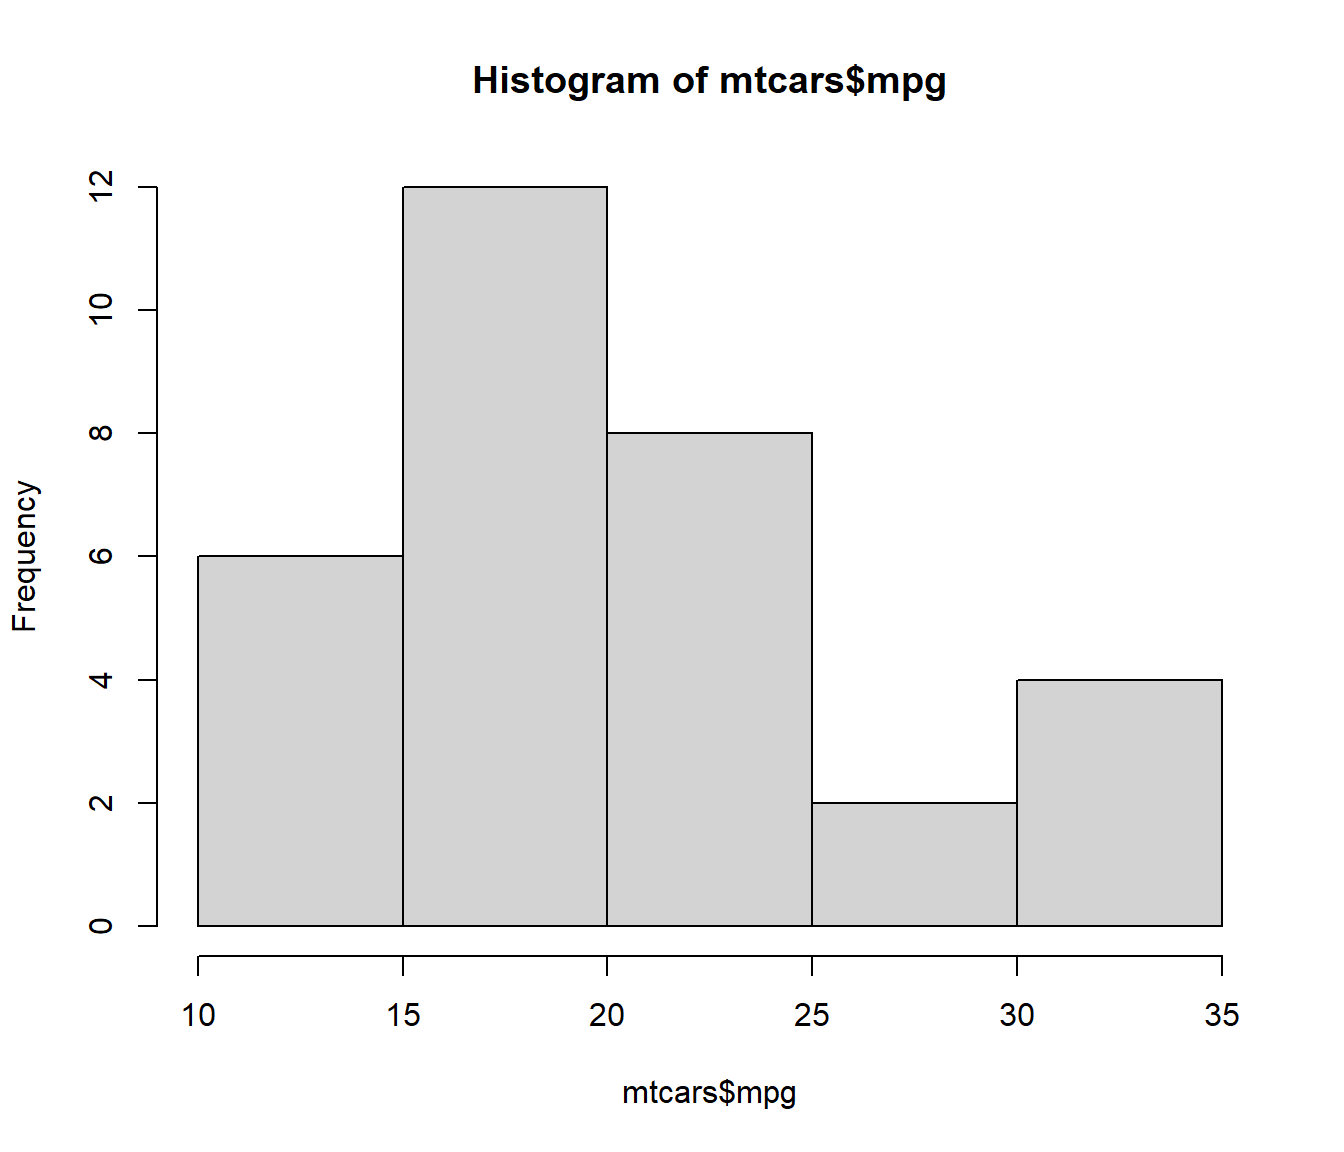
\includegraphics[width=0.8\linewidth]{08_rmarkdown_files/figure-latex/figura1-1} \end{center}

se generó empleando:

\begin{Shaded}
\begin{Highlighting}[]
\InformationTok{\textasciigrave{}\textasciigrave{}\textasciigrave{}\{r figura1, echo=FALSE\}}
\InformationTok{hist(mtcars$mpg)}
\InformationTok{\textasciigrave{}\textasciigrave{}\textasciigrave{}}
\end{Highlighting}
\end{Shaded}

aunque no se mostró previamente el código al haber establecido la opción \texttt{\textasciigrave{}\textasciigrave{}\textasciigrave{}\{r,\ echo=FALSE\}}.

\hypertarget{opcodigo}{%
\subsection{Opciones de bloques de código}\label{opcodigo}}

Los trozos de código pueden tener nombre y opciones, se establecen en la cabecera de la forma
\texttt{\textasciigrave{}\textasciigrave{}\textasciigrave{}\{r\ nombre,\ op1,\ op2\}}.
Para un listado de las opciones disponibles ver \url{http://yihui.name/knitr/options}
(en la \href{https://bookdown.org/yihui/rmarkdown/r-code.html}{Sección 2.6} del libro de RMarkdown se incluye un resumen).
En RStudio se puede pulsar en los iconos en la parte superior derecha del bloque de código para establecer opciones, ejecutar todo el código anterior o sólo el correspondiente trozo.

Algunas opciones sobre evaluación y resultados:

\begin{itemize}
\tightlist
\item
  \texttt{eval}: si \texttt{=FALSE} no se evalúa el código.
\item
  \texttt{echo}: si \texttt{=FALSE} no se muestra el código.
\item
  \texttt{include}: si \texttt{=FALSE} no se muestra el código ni ningún resultado.
\item
  \texttt{message,\ warning,\ error}: oculta el correspondiente tipo de mensaje de R
  (los errores o warnings se mostrarán en la consola).
\item
  \texttt{cache}: si se activa, guarda los resultados de la última evaluación
  y se reutilizan si no cambió el bloque de código
  (más detalles \href{https://yihui.name/knitr/options/\#cache}{aquí}).
  Puede ser de utilidad durante la redacción del documento para reducir el tiempo de renderizado
  (usándolo con cuidado y desactivándolo al terminar).
\end{itemize}

Algunas opciones sobre resultados gráficos:

\begin{itemize}
\tightlist
\item
  \texttt{fig.width,\ fig.height,\ fig.dim}: dimensiones del dispositivo gráfico de R
  (no confundir con el tamaño del resultado), e.g.~\texttt{fig.width\ =\ 5}.
\item
  \texttt{out.width,\ out.heigh}: tamaño del gráfico, e.g.~\texttt{=\textquotesingle{}80\%\textquotesingle{}}.
\item
  \texttt{fig.align}: \texttt{=\textquotesingle{}left\textquotesingle{},\ \textquotesingle{}center\textquotesingle{},\ \textquotesingle{}right\textquotesingle{}}, establece la alineación.
\item
  \texttt{fig.cap}: leyenda de la figura\footnote{Si se genera un documento en PDF/LaTeX el gráfico
    se mostrará en un entorno flotante y se puede ajustar la posición empleando la opción
    \texttt{fig.pos} (por ejemplo, \texttt{fig.pos\ =\ \textquotesingle{}!htb\textquotesingle{}}).}.
\item
  \texttt{dev}: dispositivo gráfico de R, por defecto \texttt{=\textquotesingle{}pdf\textquotesingle{}} para LaTeX y \texttt{\textquotesingle{}png\textquotesingle{}} para HTML.
  Otras opciones son \texttt{\textquotesingle{}svg\textquotesingle{}} o \texttt{\textquotesingle{}jpeg\textquotesingle{}}.
\end{itemize}

Para establecer valores por defecto para todos los bloques de código
se suele incluir uno de configuración al principio del documento, por ejemplo:

\begin{Shaded}
\begin{Highlighting}[]
\InformationTok{\textasciigrave{}\textasciigrave{}\textasciigrave{}\{r, setup, include=FALSE\}}
\InformationTok{knitr::opts\_chunk$set(comment=NA, prompt=TRUE, dev=\textquotesingle{}svg\textquotesingle{}, fig.dim=c(5, 7), collapse=TRUE)}
\InformationTok{\textasciigrave{}\textasciigrave{}\textasciigrave{}}
\end{Highlighting}
\end{Shaded}

\hypertarget{tablas}{%
\section{Tablas}\label{tablas}}

En Markdown se pueden escribir tablas en varios formatos (ver \href{https://pandoc.org/MANUAL.html\#tables}{Pandoc Tables}).
Por ejemplo:

\begin{verbatim}
  Right     Left     Center     Default
-------     ------ ----------   -------
     12     12        12            12
    123     123       123          123
      1     1          1             1   
\end{verbatim}

También:

\begin{verbatim}
Variable   | Descripción
---------  | -----------------------------------------------------------
mpg   |  Millas / galón (EE.UU.) 
cyl   |  Número de cilindros
disp  |  Desplazamiento (pulgadas cúbicas)
hp    |  Caballos de fuerza bruta
drat  |  Relación del eje trasero
wt    |  Peso (miles de libras)
qsec  |  Tiempo de 1/4 de milla
vs    |  Cilindros en V/Straight (0 = cilindros en V, 1 = cilindros en línea)
am    |  Tipo de transmisión (0 = automático, 1 = manual)
gear  |  Número de marchas (hacia adelante)
carb  |  Número de carburadores 
\end{verbatim}

que resulta en:

\begin{longtable}[]{@{}ll@{}}
\toprule
Variable & Descripción \\
\midrule
\endhead
mpg & Millas / galón (EE.UU.) \\
cyl & Número de cilindros \\
disp & Desplazamiento (pulgadas cúbicas) \\
hp & Caballos de fuerza bruta \\
drat & Relación del eje trasero \\
wt & Peso (miles de libras) \\
qsec & Tiempo de 1/4 de milla \\
vs & Cilindros en V/Straight (0 = cilindros en V, 1 = cilindros en línea) \\
am & Tipo de transmisión (0 = automático, 1 = manual) \\
gear & Número de marchas (hacia adelante) \\
carb & Número de carburadores \\
\bottomrule
\end{longtable}

Para convertir resultados de R en tablas de una forma simple se puede emplear la función \href{NA}{\texttt{ktable()}} del paquete \href{https://yihui.org/knitr/}{\texttt{knitr}}. Por ejemplo la Tabla \ref{tab:kable} se obtuvo mediante el siguiente código:

\begin{Shaded}
\begin{Highlighting}[]
\NormalTok{knitr}\SpecialCharTok{::}\FunctionTok{kable}\NormalTok{(}
  \FunctionTok{head}\NormalTok{(mtcars), }
  \AttributeTok{caption =} \StringTok{"Una kable knitr"}
\NormalTok{)}
\end{Highlighting}
\end{Shaded}

\begin{table}

\caption{\label{tab:kable}Una kable knitr}
\centering
\begin{tabular}[t]{l|r|r|r|r|r|r|r|r|r|r|r}
\hline
  & mpg & cyl & disp & hp & drat & wt & qsec & vs & am & gear & carb\\
\hline
Mazda RX4 & 21.0 & 6 & 160 & 110 & 3.90 & 2.620 & 16.46 & 0 & 1 & 4 & 4\\
\hline
Mazda RX4 Wag & 21.0 & 6 & 160 & 110 & 3.90 & 2.875 & 17.02 & 0 & 1 & 4 & 4\\
\hline
Datsun 710 & 22.8 & 4 & 108 & 93 & 3.85 & 2.320 & 18.61 & 1 & 1 & 4 & 1\\
\hline
Hornet 4 Drive & 21.4 & 6 & 258 & 110 & 3.08 & 3.215 & 19.44 & 1 & 0 & 3 & 1\\
\hline
Hornet Sportabout & 18.7 & 8 & 360 & 175 & 3.15 & 3.440 & 17.02 & 0 & 0 & 3 & 2\\
\hline
Valiant & 18.1 & 6 & 225 & 105 & 2.76 & 3.460 & 20.22 & 1 & 0 & 3 & 1\\
\hline
\end{tabular}
\end{table}

Otros paquetes proporcionan opciones adicionales: \href{http://xtable.r-forge.r-project.org/}{\texttt{xtable}}, \href{https://CRAN.R-project.org/package=stargazer}{\texttt{stargazer}}, \href{https://rapporter.github.io/pander/}{\texttt{pander}}, \href{https://r-forge.r-project.org/projects/tables/}{\texttt{tables}} y \href{https://github.com/mclements/ascii}{\texttt{ascii}}.

\hypertarget{yaml}{%
\section{Cabecera YAML}\label{yaml}}

En un fichero RMarkdown se puede incluir metadatos en una cabecera en formato YAML
(YAML Ain't Markup Language, \url{https://en.wikipedia.org/wiki/YAML}),
comenzando y terminando con tres guiones \texttt{-\/-\/-}.
Los metadatos de YAML son típicamente opciones de renderizado consitentes en
pares de etiquetas y valores separados por dos puntos.
Por ejemplo:

\begin{Shaded}
\begin{Highlighting}[]
\PreprocessorTok{{-}{-}{-}}
\FunctionTok{title}\KeywordTok{:}\AttributeTok{ }\StringTok{"Creación de contenidos con RMarkdown"}
\FunctionTok{author}\KeywordTok{:}\AttributeTok{ }\StringTok{"Fernández{-}Casal, R. y Cotos{-}Yáñez, T.R."}
\FunctionTok{date}\KeywordTok{:}\AttributeTok{ }\StringTok{"\textasciigrave{}r Sys.Date()\textasciigrave{}"}
\FunctionTok{output}\KeywordTok{:}\AttributeTok{ html\_document}
\PreprocessorTok{{-}{-}{-}}
\end{Highlighting}
\end{Shaded}

Aunque no siempre es necesario, se recomienda que los valores de texto se introduzcan entre comillas (se puede incluir código R en línea, como por ejemplo \texttt{\textasciigrave{}r\ Sys.Date()\textasciigrave{}} para obtener la fecha actual). Para valores lógicos se puede emplear \texttt{yes/true} y \texttt{no/false} para verdadero y falso, respectivamente.

Los valores pueden ser vectores, por ejemplo las siguientes opciones son equivalentes:

\begin{Shaded}
\begin{Highlighting}[]
\FunctionTok{bibliography}\KeywordTok{:}\AttributeTok{ }\KeywordTok{[}\AttributeTok{book.bib}\KeywordTok{,}\AttributeTok{ packages.bib}\KeywordTok{]}
\end{Highlighting}
\end{Shaded}

\begin{Shaded}
\begin{Highlighting}[]
\FunctionTok{bibliography}\KeywordTok{:}
\KeywordTok{{-}}\AttributeTok{ book.bib}
\KeywordTok{{-}}\AttributeTok{ packages.bib}
\end{Highlighting}
\end{Shaded}

También pueden ser listas, añadiendo una sangría de dos espacios (importante):

\begin{Shaded}
\begin{Highlighting}[]
\FunctionTok{output}\KeywordTok{:}
\AttributeTok{  }\FunctionTok{html\_document}\KeywordTok{:}
\AttributeTok{    }\FunctionTok{toc}\KeywordTok{:}\AttributeTok{ }\CharTok{yes}
\AttributeTok{    }\FunctionTok{toc\_float}\KeywordTok{:}\AttributeTok{ }\CharTok{yes}
\AttributeTok{  }\FunctionTok{pdf\_document}\KeywordTok{:}
\AttributeTok{    }\FunctionTok{toc}\KeywordTok{:}\AttributeTok{ }\CharTok{yes}
\end{Highlighting}
\end{Shaded}

El campo \texttt{output} permite especificar el formato y las opciones de salida (por defecto se empleará la primera). Empleando este campo también se pueden especificar opciones gráficas para los bloques de código, por ejemplo:

\begin{Shaded}
\begin{Highlighting}[]
\FunctionTok{output}\KeywordTok{:}
\AttributeTok{  }\FunctionTok{html\_document}\KeywordTok{:}
\AttributeTok{    }\FunctionTok{fig\_width}\KeywordTok{:}\AttributeTok{ }\DecValTok{7}
\AttributeTok{    }\FunctionTok{fig\_height}\KeywordTok{:}\AttributeTok{ }\DecValTok{6}
\AttributeTok{    }\FunctionTok{fig\_caption}\KeywordTok{:}\AttributeTok{ }\CharTok{true}
\end{Highlighting}
\end{Shaded}

La mayoría de los campos YAML son opciones que el paquete \href{https://github.com/rstudio/rmarkdown}{\texttt{rmarkdown}} le pasa a Pandoc (ver documentación en el Apéndice \ref{pandoc}).

Un ejemplo adicional\footnote{Puede ser interesante ejecutar \texttt{str(rmarkdown::html\_document())} para ver un listado de todas las opciones disponibles de \texttt{html\_document}}:

\begin{Shaded}
\begin{Highlighting}[]
\PreprocessorTok{{-}{-}{-}}
\FunctionTok{title}\KeywordTok{:}\AttributeTok{ }\StringTok{"Creación de contenidos con RMarkdown"}
\FunctionTok{subtitle}\KeywordTok{:}\AttributeTok{ }\StringTok{"Curso de introducción a R"}
\FunctionTok{author}\KeywordTok{:}
\KeywordTok{{-}}\AttributeTok{ }\FunctionTok{name}\KeywordTok{:}\AttributeTok{ }\StringTok{"Rubén Fernández Casal (ruben.fcasal@udc.es)"}
\AttributeTok{  }\FunctionTok{affiliation}\KeywordTok{:}\AttributeTok{ }\StringTok{"Universidade da Coruña"}
\KeywordTok{{-}}\AttributeTok{ }\FunctionTok{name}\KeywordTok{:}\AttributeTok{ }\StringTok{"Tomás R. Cotos Yáñez (tcotos@uvigo.es)"}
\AttributeTok{  }\FunctionTok{affiliation}\KeywordTok{:}\AttributeTok{ }\StringTok{"Universidade de Vigo"}
\FunctionTok{date}\KeywordTok{:}\AttributeTok{ }\StringTok{"2023{-}04{-}01"}
\FunctionTok{logo}\KeywordTok{:}\AttributeTok{ rmarkdown.png}
\FunctionTok{output}\KeywordTok{:}
\AttributeTok{  }\FunctionTok{html\_document}\KeywordTok{:}
\AttributeTok{    }\FunctionTok{toc}\KeywordTok{:}\AttributeTok{ }\CharTok{yes}\CommentTok{                  \# incluir tabla de contenido}
\AttributeTok{    }\FunctionTok{toc\_float}\KeywordTok{:}\AttributeTok{ }\CharTok{yes}\CommentTok{            \# toc flotante a la izquierda}
\AttributeTok{    }\FunctionTok{number\_sections}\KeywordTok{:}\AttributeTok{ }\CharTok{yes}\CommentTok{      \# numerar secciones y subsecciones}
\AttributeTok{    }\FunctionTok{code\_folding}\KeywordTok{:}\AttributeTok{ hide}\CommentTok{        \# por defecto el código aparecerá oculto}
\AttributeTok{    }\FunctionTok{mathjax}\KeywordTok{:}\AttributeTok{ local}\CommentTok{            \# emplea una copia local de MathJax, hay que establecer:}
\AttributeTok{    }\FunctionTok{self\_contained}\KeywordTok{:}\AttributeTok{ }\CharTok{false}\CommentTok{     \# las dependencias se guardan en ficheros externos}
\AttributeTok{    }\FunctionTok{lib\_dir}\KeywordTok{:}\AttributeTok{ libs}\CommentTok{             \# directorio para librerías (Bootstrap, MathJax, ...)}
\AttributeTok{  }\FunctionTok{pdf\_document}\KeywordTok{:}
\AttributeTok{    }\FunctionTok{toc}\KeywordTok{:}\AttributeTok{ }\CharTok{yes}
\AttributeTok{    }\FunctionTok{toc\_depth}\KeywordTok{:}\AttributeTok{ }\DecValTok{2}
\AttributeTok{    }\FunctionTok{keep\_tex}\KeywordTok{:}\AttributeTok{ }\CharTok{yes}\CommentTok{             \# conservar fichero latex}
\PreprocessorTok{{-}{-}{-}}
\end{Highlighting}
\end{Shaded}

Como se puede deducir del ejemplo anterior, en el formato YAML podemos incluir comentarios con el carácter \texttt{\#}
(por ejemplo para no emplear alguna de las opciones sin borrarla del encabezado).

En el \href{https://bookdown.org/yihui/rmarkdown/documents.html}{Capítulo 3} del libro de RMarkdown se tiene información detallada sobre las opciones de los distintos formatos de salida (sobre ficheros HTML en la sección \href{https://bookdown.org/yihui/rmarkdown/html-document.html}{HTML document} y sobre PDF/LaTeX en \href{https://bookdown.org/yihui/rmarkdown/pdf-document.html}{PDF document}).

\hypertarget{extracciuxf3n-del-cuxf3digo-r}{%
\section{Extracción del código R}\label{extracciuxf3n-del-cuxf3digo-r}}

Para generar un fichero con el código R se puede emplear la función \href{NA}{\texttt{knitr::ktable()}}.
Por ejemplo:

\begin{verbatim}
purl("Informe.Rmd")
\end{verbatim}

Si se quiere además el texto RMarkdown como comentarios tipo \href{https://rdrr.io/pkg/knitr/man/spin.html}{\texttt{spin()}}, se puede emplear:

\begin{verbatim}
purl("Informe.Rmd", documentation = 2)
\end{verbatim}

\hypertarget{spin}{%
\section{Spin}\label{spin}}

Una forma rápida de crear este tipo de informes a partir de un fichero de código R es emplear la función \href{https://rdrr.io/pkg/knitr/man/spin.html}{\texttt{spin()}} del paquete \href{https://yihui.org/knitr/}{\texttt{knitr}} (ver p.e. \url{https://yihui.org/knitr/demo/stitch/\#spin-comment-out-texts}).

Para ello se debe comentar todo lo que no sea código R de una forma especial:

\begin{itemize}
\item
  El texto RMarkdown se comenta con \texttt{\#\textquotesingle{}}.

  Por ejemplo:

\begin{verbatim}
#' # Este es un título de primer nivel
#' ## Este es un título de segundo nivel
\end{verbatim}
\item
  Las opciones de un trozo de código se comentan con \texttt{\#+}.

  Por ejemplo:

\begin{verbatim}
#+ setup, include=FALSE
opts_chunk$set(comment=NA, prompt=TRUE, dev='svg', fig.height=6, fig.width=6)
\end{verbatim}
\end{itemize}

Para generar el informe se puede emplear la función \href{https://rdrr.io/pkg/knitr/man/knit.html}{\texttt{knitr::purl()}}.
Por ejemplo: \texttt{spin("Ridge\_Lasso.R")}.
También se podría abrir directamente el informe generado:

\begin{verbatim}
browseURL(url = knitr::spin("Ridge_Lasso.R"))
\end{verbatim}

Pero puede ser recomendable renderizarlo con rmarkdown:

\begin{verbatim}
library(rmarkdown)
browseURL(url = render(knitr::spin("Ridge_Lasso.R", knit = FALSE)))
\end{verbatim}

En RStudio basta con pulsar \emph{Ctrl + Shift + K}, el icono correspondiente en la barra superior, o seleccionar \emph{File \textgreater{} Compile Report\ldots{}}.

Por ejemplo, si se quiere convertir la salidas de un fichero de código de R a formato LaTeX
(para añadirlas fácilmente a un documento en este formato), bastaría con incluir una cabecera de
la forma:

\begin{Shaded}
\begin{Highlighting}[]
\NormalTok{\#\textquotesingle{} {-}{-}{-}}
\NormalTok{\#\textquotesingle{} title: "Título"}
\NormalTok{\#\textquotesingle{} author: "Autor"}
\NormalTok{\#\textquotesingle{} date: "Fecha"}
\NormalTok{\#\textquotesingle{} output:}
\NormalTok{\#\textquotesingle{}   pdf\_document:}
\NormalTok{\#\textquotesingle{}      keep\_tex: true}
\NormalTok{\#\textquotesingle{} {-}{-}{-}}
\end{Highlighting}
\end{Shaded}

\hypertarget{extensiones-rmarkdown-de-pandoc}{%
\section{Extensiones RMarkdown de pandoc}\label{extensiones-rmarkdown-de-pandoc}}

Como ya se comentó, RMarkdown utiliza la sintaxis extendida proporcionada por Pandoc.
Por ejemplo, se pueden añadir sub\textsubscript{índices} y super\textsuperscript{índices} con \texttt{sub\textasciitilde{}índices\textasciitilde{}} y \texttt{super\^{}índices\^{}},\\
y notas al pie con \texttt{\^{}{[}texto{]}}.

Podemos incluir expresiones matemáticas en formato LateX (ver e.g.~\href{https://www.overleaf.com/learn/latex/Free_online_introduction_to_LaTeX_(part_1)}{Free online introduction to LaTeX}):

\begin{itemize}
\item
  En linea escribiendo la expresión latex entre dos símbolos de dolar,
  por ejemplo \texttt{\$\textbackslash{}alpha,\ \textbackslash{}beta,\ \textbackslash{}gamma,\ \textbackslash{}delta\$}
  resultaría en \(\alpha, \beta, \gamma, \delta\).
\item
  En formato ecuación empleando dos pares de símbolos de dolar. Por ejemplo:
  \texttt{\$\$\textbackslash{}Theta\ =\ \textbackslash{}begin\{pmatrix\}\textbackslash{}alpha\ \&\ \textbackslash{}beta\textbackslash{}\textbackslash{}\ \ \ \ \ \textbackslash{}gamma\ \&\ \textbackslash{}delta\ \ \ \ \ \textbackslash{}end\{pmatrix\}\$\$}
  resultaría en:
  \[\Theta = \begin{pmatrix}\alpha & \beta\\
  \gamma & \delta
  \end{pmatrix}\]
\end{itemize}

También admite bibliografía, ver p.e. \href{https://pandoc.org/MANUAL.html\#citations}{Pandoc Citations}.
Lo más cómodo puede ser emplear un archivo de bibliografía en formato BibTeX, lo que se describe con detalle en \href{https://bookdown.org/yihui/bookdown/citations.html}{Citations}.
Será necesario añadir un campo \texttt{bibliography} en la cabezera YAML, por ejemplo:

\begin{Shaded}
\begin{Highlighting}[]
\FunctionTok{bibliography}\KeywordTok{:}\AttributeTok{ bibliografia.bib}
\FunctionTok{csl}\KeywordTok{:}\AttributeTok{ apa.csl}\CommentTok{  \# opcional}
\end{Highlighting}
\end{Shaded}

Suponiendo que en el directorio de trabajo están los ficheros de bibliografía \emph{bibliografia.bib}
y de estilo \emph{apa.csl} (ver \url{http://citationstyles.org/}, desde donde se pueden descargar
distintos archivos de estilo).

Las referencias en el texto RMarkdown se incluyen con \texttt{@referencia} o \texttt{{[}@referencia{]}}.
Pandoc generará el listado de referencias al final del documento,
por lo que nos puede interesar insertar una última sección \texttt{\#\ Bibliografía\ \{-\}}
al generar documentos HTML (en PDF se hará automáticamente al emplear LaTeX).
En RStudio se puede instalar el ``\href{https://rstudio.github.io/rstudioaddins/}{Addin}''
\href{https://github.com/crsh/citr}{\texttt{citr}} para insertar
citas a referencias bibliográficas en formato BibTeX.

Para más detalles de las extensiones de Pandoc ver por ejemplo \href{https://pandoc.org/MANUAL.html\#pandocs-markdown}{Pandoc's Markdown}.

\hypertarget{part-tidyverse}{%
\part{Tidyverse}\label{part-tidyverse}}

\hypertarget{tidyverse}{%
\chapter{El ecosistema tidyverse}\label{tidyverse}}

En los capítulos de esta parte se pretende realizar una breve introducción al \emph{ecosistema} \href{https://dplyr.tidyverse.org}{\textbf{Tidyverse}}, una colección de paquetes diseñados de forma uniforme (con la misma filosofía y estilo) para trabajar conjuntamente.

La referencia recomendada para usuarios de R que deseen iniciarse en el uso de estos paquetes es:

Wickham, H., y Grolemund, G. (2016). \emph{\href{http://r4ds.had.co.nz}{R for data science: import, tidy, transform, visualize, and model data}}, \href{https://es.r4ds.hadley.nz}{online-castellano}, \href{http://shop.oreilly.com/product/0636920034407.do}{O'Reilly}.

El paquete \href{https://tidyverse.tidyverse.org}{\texttt{tidyverse}} está diseñado para facilitar la instalación y carga de los paquetes principales de la colección tidyverse con un solo comando.
Al instalar este paquete se instalan paquetes que forman el denominado núcleo de tidyverse (se cargan con \texttt{library(tidyverse)}):

\begin{itemize}
\tightlist
\item
  \href{https://ggplot2.tidyverse.org}{\texttt{ggplot2}}: visualización de datos.
\item
  \href{https://dplyr.tidyverse.org}{\texttt{dplyr}}: manipulación de datos.
\item
  \href{https://tidyr.tidyverse.org}{\texttt{tidyr}}: reorganización (limpieza) de datos.
\item
  \href{https://readr.tidyverse.org}{\texttt{readr}}: importación de datos.
\item
  \href{https://tibble.tidyverse.org}{\texttt{tibble}}: tablas de datos (extensión de \texttt{data.frame}).
\item
  \href{https://purrr.tidyverse.org}{\texttt{purrr}}: programación funcional.
\item
  \href{https://github.com/tidyverse/stringr}{\texttt{stringr}}: manipulación de cadenas de texto.
\item
  \href{https://github.com/tidyverse/forcats}{\texttt{forcats}}: manipulación de factores.
\item
  \href{https://github.com/tidyverse/lubridate}{\texttt{lubridate}}: manipulación de fechas y horas.
\end{itemize}

y un conjunto de paquetes recomendados (\href{https://github.com/wesm/feather}{\texttt{feather}}, \href{https://github.com/tidyverse/haven}{\texttt{haven}}, \href{https://github.com/tidyverse/modelr}{\texttt{modelr}}, \href{https://github.com/tidymodels/broom}{\texttt{broom}}\ldots), entre los que destacaría:

\begin{itemize}
\tightlist
\item
  \href{https://github.com/tidyverse/readxl}{\texttt{readxl}}: archivos excel.
\item
  \href{https://github.com/tidyverse/hms}{\texttt{hms}}: manipulación de medidas de tiempo.
\item
  \href{https://github.com/r-lib/httr}{\texttt{httr}}: web APIs.
\item
  \href{https://github.com/jeroen/jsonlite}{\texttt{jsonlite}}: archivos JSON.
\item
  \href{https://github.com/tidyverse/rvest}{\texttt{rvest}}: web scraping.
\item
  \href{https://github.com/r-lib/xml2}{\texttt{xml2}}: archivos XML.
\end{itemize}

\begin{Shaded}
\begin{Highlighting}[]
\FunctionTok{library}\NormalTok{(tidyverse)}
\end{Highlighting}
\end{Shaded}

También hay paquetes ``asociados'':

\begin{itemize}
\tightlist
\item
  \href{https://rlang.r-lib.org}{\texttt{rlang}}
\item
  \href{https://tidyselect.r-lib.org}{\texttt{tidyselect}}
\item
  \href{https://tidymodels.tidymodels.org}{\texttt{tidymodels}}
\end{itemize}

Muchos otros paquetes están adaptando este estilo (ver e.g.~\href{https://tidyverts.org/}{tidyverts}): \href{https://fable.tidyverts.org}{\texttt{fable}}, \href{https://r-spatial.github.io/sf/}{\texttt{sf}}\ldots{}

Resumiendo, está muy de moda y puede terminar convirtiéndose en un dialecto del lenguaje R\ldots{} para mi ya lo es\ldots{} todo lo que resulte de utilidad es bien venido\ldots{} Recomiendo evitar estos paquetes en las primeras etapas de formación en R\ldots{}

El estilo de programación tiene como origen la gramática de \href{https://ggplot2.tidyverse.org}{\texttt{ggplot2}} para crear gráficos de forma declarativa, basado a su vez en:

Wilkinson, L. (2005). \emph{The Grammar of Graphics}. \href{https://www.google.es/books/edition/The_Grammar_of_Graphics/YGgUswEACAAJ?hl=es}{Springer}.

Yo empleo este paquete como sustituto de los gráficos \href{http://lattice.r-forge.r-project.org/}{\texttt{lattice}}, en algunos informes finales o aplicaciones para empresas, o para gráficos muy especializados.
En condiciones normales \textbf{prefiero emplear los gráficos estándar} de R (mucho más rápidos de generar y programar).

Para iniciarse en este paquete lo recomendado es consultar los capítulos \href{https://r4ds.had.co.nz/data-visualisation.html}{Data Visualización} y \href{https://r4ds.had.co.nz/graphics-for-communication.html}{Graphics for communication} de \href{https://r4ds.had.co.nz}{R for Data Science}.
También puede resultar de interés la \href{https://github.com/rstudio/cheatsheets/blob/master/data-visualization.pdf}{chuleta}).
La referencia que cubre con mayor profundidad este paquete es:

Wickham, H. (2016). \emph{\href{https://ggplot2-book.org}{ggplot2: Elegant graphics for Data Analysis}} (3ª edición, en desarrollo junto a Navarro, D. y Pedersen, T.L.). \href{https://www.amazon.com/gp/product/331924275X}{Springer}.

Aunque yo recomendaría:

Chang, W. (2023). \emph{\href{https://r-graphics.org}{The R Graphics Cookbook}}. \href{https://www.amazon.com/dp/1491978600}{O'Reilly}.

En \href{https://ggplot2.tidyverse.org}{\texttt{ggplot2}} se emplea el operador \texttt{+} para añadir componentes de los gráficos (ver , en \emph{Tidyverse} se emplea un operador de redirección para añadir operaciones.

\hypertarget{pipe}{%
\section{\texorpdfstring{Operador \emph{pipe} (redirección)}{Operador pipe (redirección)}}\label{pipe}}

El operador \texttt{\%\textgreater{}\%} (paquete \href{https://magrittr.tidyverse.org}{\texttt{magrittr}}) permite canalizar la salida de una función a la entrada de otra.
Por ejemplo, \texttt{segundo(primero(datos))} se traduce en \texttt{datos\ \%\textgreater{}\%\ primero\ \%\textgreater{}\%\ segundo}, lo que facilita la lectura de operaciones al escribir las funciones de izquierda a derecha.

Desde la versión 4.1 de R está disponible un operador interno \texttt{\textbar{}\textgreater{}} (aunque yo sigo prefiriendo \texttt{\%\textgreater{}\%}).
Por ejemplo:

\begin{Shaded}
\begin{Highlighting}[]
\CommentTok{\# El fichero \textquotesingle{}empleados.RData\textquotesingle{} contiene datos de empleados de un banco.}
\CommentTok{\# Supongamos por ejemplo que estamos interesados en estudiar si hay}
\CommentTok{\# discriminación por cuestión de sexo o raza.}

\FunctionTok{load}\NormalTok{(}\StringTok{"datos/empleados.RData"}\NormalTok{)}
\CommentTok{\# NOTA: Cuidado con la codificación latin1 (no declarada) }
\CommentTok{\# al abrir archivos creados en versiones anteriores de R \textless{} 4.2: }
\CommentTok{\# load("datos/empleados.latin1.RData")}

\CommentTok{\# Listamos las etiquetas}
\NormalTok{knitr}\SpecialCharTok{::}\FunctionTok{kable}\NormalTok{(}\FunctionTok{attr}\NormalTok{(empleados, }\StringTok{"variable.labels"}\NormalTok{), }\AttributeTok{col.names =} \StringTok{"Etiqueta"}\NormalTok{)}
\end{Highlighting}
\end{Shaded}

\begin{tabular}{l|l}
\hline
  & Etiqueta\\
\hline
id & Código de empleado\\
\hline
sexo & Sexo\\
\hline
fechnac & Fecha de nacimiento\\
\hline
educ & Nivel educativo  (años)\\
\hline
catlab & Categoría laboral\\
\hline
salario & Salario actual\\
\hline
salini & Salario inicial\\
\hline
tiempemp & Meses desde el contrato\\
\hline
expprev & Experiencia previa (meses)\\
\hline
minoria & Clasificación étnica\\
\hline
sexoraza & Clasificación por sexo y raza\\
\hline
\end{tabular}

\begin{Shaded}
\begin{Highlighting}[]
\CommentTok{\# Eliminamos las etiquetas para que no molesten...}
\CommentTok{\# attr(empleados, "variable.labels") \textless{}{-} NULL  }

\NormalTok{empleados }\SpecialCharTok{|}\ErrorTok{\textgreater{}}  \FunctionTok{subset}\NormalTok{(catlab }\SpecialCharTok{==} \StringTok{"Directivo"}\NormalTok{, catlab}\SpecialCharTok{:}\NormalTok{sexoraza) }\SpecialCharTok{|}\ErrorTok{\textgreater{}}  \FunctionTok{summary}\NormalTok{()}
\end{Highlighting}
\end{Shaded}

\begin{verbatim}
##             catlab      salario           salini         tiempemp    
##  Administrativo: 0   Min.   : 34410   Min.   :15750   Min.   :64.00  
##  Seguridad     : 0   1st Qu.: 51956   1st Qu.:23063   1st Qu.:73.00  
##  Directivo     :84   Median : 60500   Median :28740   Median :81.00  
##                      Mean   : 63978   Mean   :30258   Mean   :81.15  
##                      3rd Qu.: 71281   3rd Qu.:34058   3rd Qu.:91.00  
##                      Max.   :135000   Max.   :79980   Max.   :98.00  
##     expprev       minoria          sexoraza 
##  Min.   :  3.00   No:80   Blanca varón :70  
##  1st Qu.: 19.75   Sí: 4   Blanca mujer : 4  
##  Median : 52.00           Minoría varón:10  
##  Mean   : 77.62           Minoría mujer: 0  
##  3rd Qu.:125.25                             
##  Max.   :285.00
\end{verbatim}

Para que una función sea compatible con este tipo de operadores el primer parámetro debería ser siempre los datos.
Sin embargo, el operador \texttt{\%\textgreater{}\%} permite redirigir el resultado de la operación anterior a un parámetro distinto mediante un \texttt{.}.
Por ejemplo:

\begin{Shaded}
\begin{Highlighting}[]
\CommentTok{\# ?"|\textgreater{}"}
\CommentTok{\# empleados |\textgreater{} subset(catlab != "Seguridad") |\textgreater{} droplevels |\textgreater{} }
\CommentTok{\#     boxplot(salario \textasciitilde{} sexo*catlab, data = .) \# ERROR}

\FunctionTok{library}\NormalTok{(magrittr)}
\NormalTok{empleados }\SpecialCharTok{\%\textgreater{}\%} \FunctionTok{subset}\NormalTok{(catlab }\SpecialCharTok{!=} \StringTok{"Seguridad"}\NormalTok{) }\SpecialCharTok{\%\textgreater{}\%} \FunctionTok{droplevels}\NormalTok{() }\SpecialCharTok{\%\textgreater{}\%}
    \FunctionTok{boxplot}\NormalTok{(salario }\SpecialCharTok{\textasciitilde{}}\NormalTok{ sexo}\SpecialCharTok{*}\NormalTok{catlab, }\AttributeTok{data =}\NormalTok{ .)}
\end{Highlighting}
\end{Shaded}

\begin{center}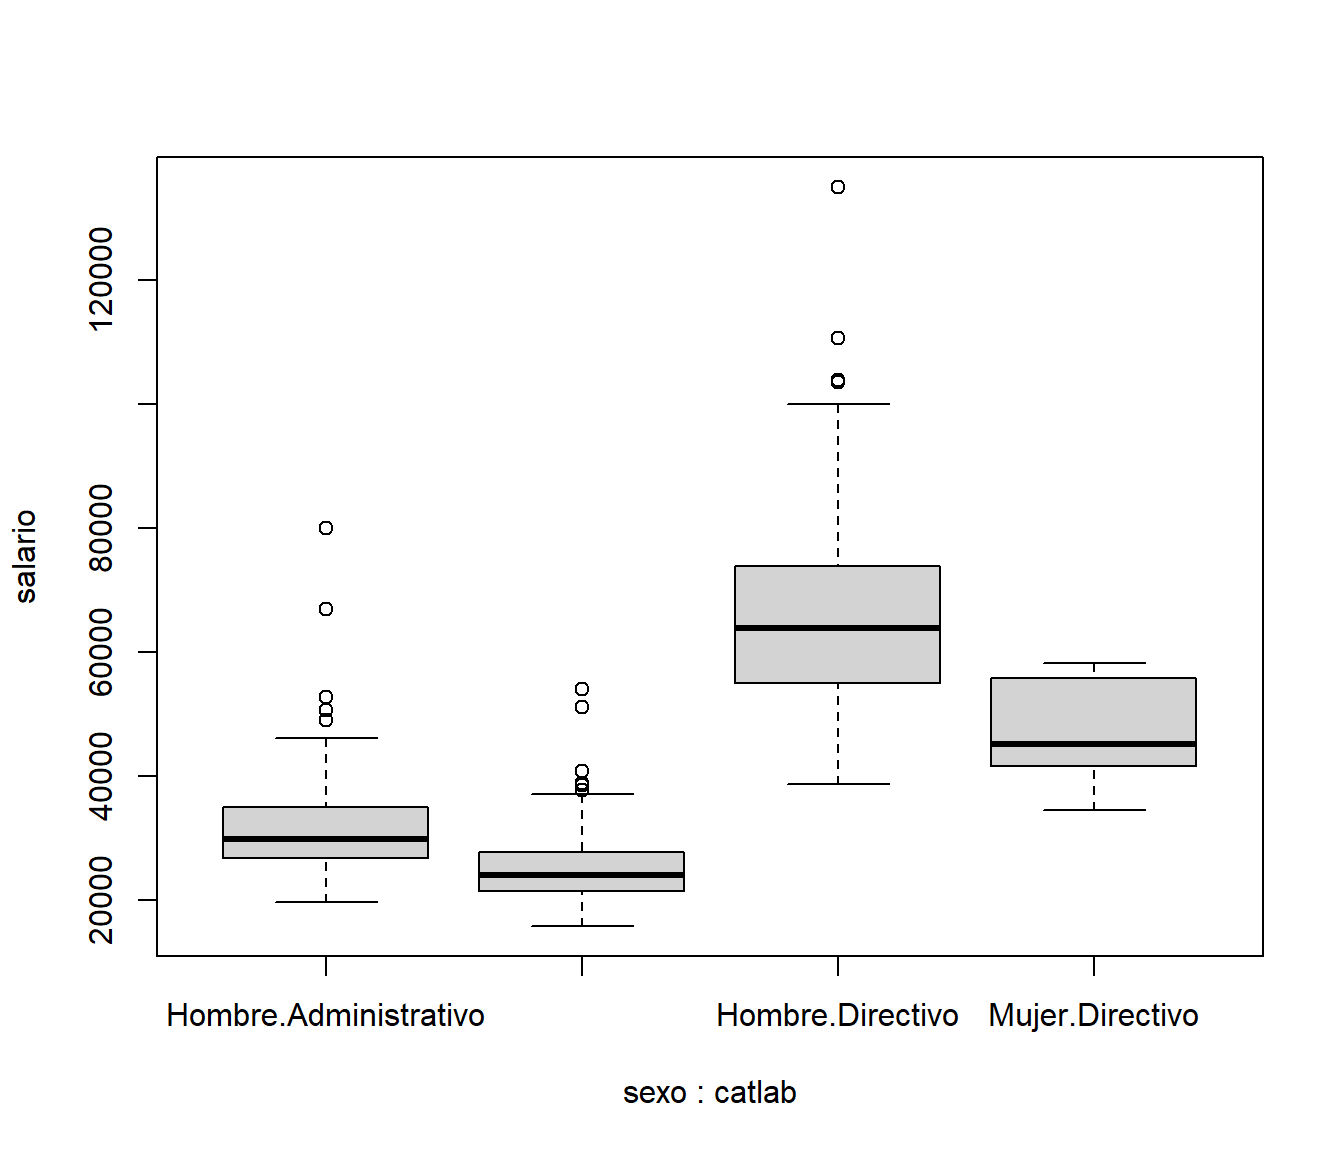
\includegraphics[width=0.8\linewidth]{10_tidyverse_files/figure-latex/unnamed-chunk-3-1} \end{center}

\hypertarget{dplyr}{%
\chapter{Manipulación de datos con dplyr y tidyr}\label{dplyr}}

En este capítulo se realiza una breve introducción al paquete \href{https://dplyr.tidyverse.org}{\texttt{dplyr}} y se comentan algunas de las utilidades del paquete \href{https://tidyr.tidyverse.org}{\texttt{tidyr}} que pueden resultar de interés\footnote{Otra alternativa (más rápida) es \href{https://rdatatable.gitlab.io/data.table}{\texttt{data.table}} pero en versiones recientes ya se puede emplear desde \texttt{dplyr}, como se comenta más adelante.}.

La referencia recomendada para iniciarse en esta herramienta es el Capítulo \href{http://r4ds.had.co.nz/transform.html}{5 Data transformation} de
\href{http://r4ds.had.co.nz}{R for Data Science}.
También puede resultar de utilidad la viñeta del paquete \href{https://dplyr.tidyverse.org/articles/dplyr.html}{Introduction to dplyr} o la \href{https://posit.co/wp-content/uploads/2022/10/data-transformation-1.pdf}{chuleta} (menú de RStudio \emph{Help \textgreater{} Cheat Sheets \textgreater{} Data Transformation with dplyr}).

\hypertarget{dplyr-pkg}{%
\section{El paquete dplyr}\label{dplyr-pkg}}

\begin{Shaded}
\begin{Highlighting}[]
\FunctionTok{library}\NormalTok{(dplyr)}
\end{Highlighting}
\end{Shaded}

La principal ventaja de \href{https://dplyr.tidyverse.org/index.html}{\texttt{dplyr}} es que permite trabajar (de la misma forma) con datos en distintos formatos:

\begin{itemize}
\item
  \texttt{data.frame}, \href{https://tibble.tidyverse.org/}{\texttt{tibble}}.
\item
  \href{https://rdatatable.gitlab.io/data.table}{\texttt{data.table}}: extensión (paquete \emph{backend}) \href{https://dtplyr.tidyverse.org}{\texttt{dtplyr}}.
\item
  conjuntos de datos más grandes que la memoria disponible: extensiones \href{https://duckdb.org/docs/api/r}{\texttt{duckdb}} y \href{https://arrow.apache.org/docs/r/}{\texttt{arrow}} (incluyendo almacenamiento en la nube, e.g.~\href{https://aws.amazon.com/es/s3}{AWS}).
\item
  bases de datos relacionales (lenguaje SQL, locales o remotas); extensión \href{https://dbplyr.tidyverse.org}{\texttt{dbplyr}}.
\item
  grandes volúmenes de datos (incluso almacenados en múltiples servidores; ecosistema \href{http://hadoop.apache.org/}{Hadoop}/\href{https://spark.apache.org/}{Spark}): extensión \href{https://spark.rstudio.com}{\texttt{sparklyr}} (ver menú de RStudio \emph{Help \textgreater{} Cheat Sheets \textgreater{} Interfacing Spark with sparklyr}).
\end{itemize}

El paquete dplyr permite sustituir operaciones con funciones base de R (como \href{NA}{\texttt{subset}}, \href{NA}{\texttt{split}}, \href{NA}{\texttt{apply}}, \href{NA}{\texttt{sapply}}, \href{NA}{\texttt{lapply}}, \href{NA}{\texttt{tapply}}, \href{NA}{\texttt{aggregate}}\ldots) por una ``gramática'' más sencilla para la manipulación de datos.
En lugar de operar sobre vectores como la mayoría de las funciones base,
opera sobre conjuntos de datos (de forma que es compatible con el operador \texttt{\%\textgreater{}\%}).
Los principales ``verbos'' (funciones) son:

\begin{itemize}
\item
  \href{https://dplyr.tidyverse.org/reference/select.html}{\texttt{select()}}: seleccionar variables (ver también \href{https://dplyr.tidyverse.org/reference/rename.html}{\texttt{rename}}, \href{https://dplyr.tidyverse.org/reference/rename.html}{\texttt{relocate}}, \href{https://dplyr.tidyverse.org/reference/rename.html}{\texttt{pull}}).
\item
  \href{https://dplyr.tidyverse.org/reference/mutate.html}{\texttt{mutate()}}: crear variables (ver también \texttt{transmute()}).
\item
  \href{https://dplyr.tidyverse.org/reference/filter.html}{\texttt{filter()}}: seleccionar casos/filas (ver también \texttt{slice()}).
\item
  \href{https://dplyr.tidyverse.org/reference/arrange.html}{\texttt{arrange()}}: ordenar casos/filas.
\item
  \href{https://dplyr.tidyverse.org/reference/summarise.html}{\texttt{summarise()}}: resumir valores.
\item
  \href{https://dplyr.tidyverse.org/reference/group_by.html}{\texttt{group\_by()}}: permite operaciones por grupo empleando el concepto ``dividir-aplicar-combinar'' (\texttt{ungroup()} elimina el agrupamiento).
\end{itemize}

NOTA: Para entender el funcionamiento de ciertas funciones (como \href{https://dplyr.tidyverse.org/reference/rowwise.html}{\texttt{rowwise()}}) y las posibilidades en el manejo de datos, hay que tener en cuenta que un \texttt{data.frame} no es más que una lista cuyas componentes (variables) tienen la misma longitud.
Realmente las componentes también pueden ser listas de la misma longitud y, por tanto, podemos almacenar casi cualquier estructura de datos en un \texttt{data.frame}.

En la primera parte de este capítulo consideraremos solo \texttt{data.frame} por comodidad.
Emplearemos como ejemplo los datos de empleados de banca almacenados en el fichero \emph{empleados.RData} (y supondremos que estamos interesados en estudiar si hay discriminación por cuestión de sexo o raza).

\begin{Shaded}
\begin{Highlighting}[]
\FunctionTok{load}\NormalTok{(}\StringTok{"datos/empleados.RData"}\NormalTok{)}
\FunctionTok{attr}\NormalTok{(empleados, }\StringTok{"variable.labels"}\NormalTok{) }\OtherTok{\textless{}{-}} \ConstantTok{NULL}                  
\end{Highlighting}
\end{Shaded}

En la Sección \ref{dbplyr} final emplearemos una base de datos relacional como ejemplo.

\hypertarget{dplyr-variables}{%
\section{Operaciones con variables (columnas)}\label{dplyr-variables}}

Podemos \textbf{seleccionar variables con \href{https://dplyr.tidyverse.org/reference/select.html}{\texttt{select()}}}:

\begin{Shaded}
\begin{Highlighting}[]
\NormalTok{emplea2 }\OtherTok{\textless{}{-}}\NormalTok{ empleados }\SpecialCharTok{\%\textgreater{}\%} \FunctionTok{select}\NormalTok{(id, sexo, minoria, tiempemp, salini, salario)}
\FunctionTok{head}\NormalTok{(emplea2)}
\end{Highlighting}
\end{Shaded}

\begin{verbatim}
##   id   sexo minoria tiempemp salini salario
## 1  1 Hombre      No       98  27000   57000
## 2  2 Hombre      No       98  18750   40200
## 3  3  Mujer      No       98  12000   21450
## 4  4  Mujer      No       98  13200   21900
## 5  5 Hombre      No       98  21000   45000
## 6  6 Hombre      No       98  13500   32100
\end{verbatim}

Se puede cambiar el nombre (ver también \href{https://dplyr.tidyverse.org/reference/rename.html}{\texttt{rename()}}):

\begin{Shaded}
\begin{Highlighting}[]
\NormalTok{empleados }\SpecialCharTok{\%\textgreater{}\%} \FunctionTok{select}\NormalTok{(sexo, }\AttributeTok{noblanca =}\NormalTok{ minoria, salario) }\SpecialCharTok{\%\textgreater{}\%} \FunctionTok{head}\NormalTok{()}
\end{Highlighting}
\end{Shaded}

\begin{verbatim}
##     sexo noblanca salario
## 1 Hombre       No   57000
## 2 Hombre       No   40200
## 3  Mujer       No   21450
## 4  Mujer       No   21900
## 5 Hombre       No   45000
## 6 Hombre       No   32100
\end{verbatim}

Se pueden emplear los nombres de variables como índices:

\begin{Shaded}
\begin{Highlighting}[]
\NormalTok{empleados }\SpecialCharTok{\%\textgreater{}\%} \FunctionTok{select}\NormalTok{(sexo}\SpecialCharTok{:}\NormalTok{salario) }\SpecialCharTok{\%\textgreater{}\%} \FunctionTok{head}\NormalTok{()}
\end{Highlighting}
\end{Shaded}

\begin{verbatim}
##     sexo    fechnac educ         catlab salario
## 1 Hombre 1952-02-03   15      Directivo   57000
## 2 Hombre 1958-05-23   16 Administrativo   40200
## 3  Mujer 1929-07-26   12 Administrativo   21450
## 4  Mujer 1947-04-15    8 Administrativo   21900
## 5 Hombre 1955-02-09   15 Administrativo   45000
## 6 Hombre 1958-08-22   15 Administrativo   32100
\end{verbatim}

\begin{Shaded}
\begin{Highlighting}[]
\CommentTok{\# empleados \%\textgreater{}\% select({-}(sexo:salario)) \%\textgreater{}\% head()}
\NormalTok{empleados }\SpecialCharTok{\%\textgreater{}\%} \FunctionTok{select}\NormalTok{(}\SpecialCharTok{!}\NormalTok{(sexo}\SpecialCharTok{:}\NormalTok{salario)) }\SpecialCharTok{\%\textgreater{}\%} \FunctionTok{head}\NormalTok{()}
\end{Highlighting}
\end{Shaded}

\begin{verbatim}
##   id salini tiempemp expprev minoria      sexoraza
## 1  1  27000       98     144      No  Blanca varón
## 2  2  18750       98      36      No  Blanca varón
## 3  3  12000       98     381      No Minoría varón
## 4  4  13200       98     190      No Minoría varón
## 5  5  21000       98     138      No  Blanca varón
## 6  6  13500       98      67      No  Blanca varón
\end{verbatim}

Se pueden emplear distintas herramientas (\emph{\href{https://tidyselect.r-lib.org/reference/language.html}{selection helpers}}) para seleccionar variables (ver paquete \href{https://tidyselect.r-lib.org}{\texttt{tidyselect}}):

\begin{itemize}
\item
  \href{https://tidyselect.r-lib.org/reference/starts_with.html}{\texttt{starts\_with}}, \href{https://tidyselect.r-lib.org/reference/starts_with.html}{\texttt{ends\_with}}, \href{https://tidyselect.r-lib.org/reference/starts_with.html}{\texttt{contains}}, \href{https://tidyselect.r-lib.org/reference/starts_with.html}{\texttt{matches}}, \href{https://tidyselect.r-lib.org/reference/starts_with.html}{\texttt{num\_range}}: variables que coincidan con un patrón.
\item
  \href{https://tidyselect.r-lib.org/reference/all_of.html}{\texttt{all\_of}}, \href{https://tidyselect.r-lib.org/reference/all_of.html}{\texttt{any\_of}}: variables de un vectores de caracteres.
\item
  \href{https://tidyselect.r-lib.org/reference/everything.html}{\texttt{everything}}, \href{https://tidyselect.r-lib.org/reference/everything.html}{\texttt{last\_col}}: todas las variables o la última variable.
\item
  \href{https://tidyselect.r-lib.org/reference/where.html}{\texttt{where()}}: a partir de una función (e.g.~\texttt{where(is.numeric)})
\end{itemize}

Por ejemplo:

\begin{Shaded}
\begin{Highlighting}[]
\NormalTok{empleados }\SpecialCharTok{\%\textgreater{}\%} \FunctionTok{select}\NormalTok{(}\FunctionTok{starts\_with}\NormalTok{(}\StringTok{"s"}\NormalTok{)) }\SpecialCharTok{\%\textgreater{}\%} \FunctionTok{head}\NormalTok{()}
\end{Highlighting}
\end{Shaded}

\begin{verbatim}
##     sexo salario salini      sexoraza
## 1 Hombre   57000  27000  Blanca varón
## 2 Hombre   40200  18750  Blanca varón
## 3  Mujer   21450  12000 Minoría varón
## 4  Mujer   21900  13200 Minoría varón
## 5 Hombre   45000  21000  Blanca varón
## 6 Hombre   32100  13500  Blanca varón
\end{verbatim}

Podemos \textbf{crear variables con \href{https://dplyr.tidyverse.org/reference/mutate.html}{\texttt{mutate()}}}:

\begin{Shaded}
\begin{Highlighting}[]
\NormalTok{emplea2 }\SpecialCharTok{\%\textgreater{}\%} \FunctionTok{mutate}\NormalTok{(}\AttributeTok{incsal =}\NormalTok{ salario }\SpecialCharTok{{-}}\NormalTok{ salini, }\AttributeTok{tsal =}\NormalTok{ incsal}\SpecialCharTok{/}\NormalTok{tiempemp) }\SpecialCharTok{\%\textgreater{}\%} \FunctionTok{head}\NormalTok{()}
\end{Highlighting}
\end{Shaded}

\begin{verbatim}
##   id   sexo minoria tiempemp salini salario incsal      tsal
## 1  1 Hombre      No       98  27000   57000  30000 306.12245
## 2  2 Hombre      No       98  18750   40200  21450 218.87755
## 3  3  Mujer      No       98  12000   21450   9450  96.42857
## 4  4  Mujer      No       98  13200   21900   8700  88.77551
## 5  5 Hombre      No       98  21000   45000  24000 244.89796
## 6  6 Hombre      No       98  13500   32100  18600 189.79592
\end{verbatim}

\hypertarget{dplyr-casos}{%
\section{Operaciones con casos (filas)}\label{dplyr-casos}}

Podemos \textbf{seleccionar casos con \href{https://dplyr.tidyverse.org/reference/filter.html}{\texttt{filter()}}}:

\begin{Shaded}
\begin{Highlighting}[]
\NormalTok{emplea2 }\SpecialCharTok{\%\textgreater{}\%} \FunctionTok{filter}\NormalTok{(sexo }\SpecialCharTok{==} \StringTok{"Mujer"}\NormalTok{, minoria }\SpecialCharTok{==} \StringTok{"Sí"}\NormalTok{) }\SpecialCharTok{\%\textgreater{}\%} \FunctionTok{head}\NormalTok{()}
\end{Highlighting}
\end{Shaded}

\begin{verbatim}
##   id  sexo minoria tiempemp salini salario
## 1 14 Mujer      Sí       98  16800   35100
## 2 23 Mujer      Sí       97  11100   24000
## 3 24 Mujer      Sí       97   9000   16950
## 4 25 Mujer      Sí       97   9000   21150
## 5 40 Mujer      Sí       96   9000   19200
## 6 41 Mujer      Sí       96  11550   23550
\end{verbatim}

Podemos \textbf{reordenar casos con \href{https://dplyr.tidyverse.org/reference/arrange.html}{\texttt{arrange()}}}:

\begin{Shaded}
\begin{Highlighting}[]
\NormalTok{emplea2 }\SpecialCharTok{\%\textgreater{}\%} \FunctionTok{arrange}\NormalTok{(salario) }\SpecialCharTok{\%\textgreater{}\%} \FunctionTok{head}\NormalTok{()}
\end{Highlighting}
\end{Shaded}

\begin{verbatim}
##    id  sexo minoria tiempemp salini salario
## 1 378 Mujer      No       70  10200   15750
## 2 338 Mujer      No       74  10200   15900
## 3  90 Mujer      No       92   9750   16200
## 4 224 Mujer      No       82  10200   16200
## 5 411 Mujer      No       68  10200   16200
## 6 448 Mujer      Sí       66  10200   16350
\end{verbatim}

\begin{Shaded}
\begin{Highlighting}[]
\NormalTok{emplea2 }\SpecialCharTok{\%\textgreater{}\%} \FunctionTok{arrange}\NormalTok{(}\FunctionTok{desc}\NormalTok{(salini), salario) }\SpecialCharTok{\%\textgreater{}\%} \FunctionTok{head}\NormalTok{()}
\end{Highlighting}
\end{Shaded}

\begin{verbatim}
##    id   sexo minoria tiempemp salini salario
## 1  29 Hombre      No       96  79980  135000
## 2 343 Hombre      No       73  60000  103500
## 3 205 Hombre      No       83  52500   66750
## 4 160 Hombre      No       86  47490   66000
## 5 431 Hombre      No       66  45000   86250
## 6  32 Hombre      No       96  45000  110625
\end{verbatim}

Podemos \textbf{resumir valores con \href{https://dplyr.tidyverse.org/reference/summarise.html}{\texttt{summarise()}}}:

\begin{Shaded}
\begin{Highlighting}[]
\NormalTok{empleados }\SpecialCharTok{\%\textgreater{}\%} \FunctionTok{summarise}\NormalTok{(}\AttributeTok{sal.med =} \FunctionTok{mean}\NormalTok{(salario), }\AttributeTok{n =} \FunctionTok{n}\NormalTok{())}
\end{Highlighting}
\end{Shaded}

\begin{verbatim}
##    sal.med   n
## 1 34419.57 474
\end{verbatim}

Para realizar \textbf{operaciones con múltiples variables podemos emplear \href{https://dplyr.tidyverse.org/reference/across.html}{\texttt{across()}}} (admite selección de variables \href{https://tidyselect.r-lib.org}{\texttt{tidyselect}}):

\begin{Shaded}
\begin{Highlighting}[]
\NormalTok{empleados }\SpecialCharTok{\%\textgreater{}\%} \FunctionTok{summarise}\NormalTok{(}\FunctionTok{across}\NormalTok{(}\FunctionTok{where}\NormalTok{(is.numeric), mean), }\AttributeTok{n =} \FunctionTok{n}\NormalTok{())}
\end{Highlighting}
\end{Shaded}

\begin{verbatim}
##      id     educ  salario   salini tiempemp  expprev   n
## 1 237.5 13.49156 34419.57 17016.09  81.1097 95.86076 474
\end{verbatim}

\begin{Shaded}
\begin{Highlighting}[]
\CommentTok{\# empleados \%\textgreater{}\% summarise(across(where(is.numeric) \& !id, mean), n = n())}
\end{Highlighting}
\end{Shaded}

NOTA: Esta función sustituye a las ``variantes de ámbito'' \texttt{\_at()}, \texttt{\_if()} y \texttt{\_all()} de versiones anteriores de dplyr (como \texttt{summarise\_at()}, \texttt{summarise\_if()}, \texttt{summarise\_all()}, \texttt{mutate\_at()}, \texttt{mutate\_if()}\ldots) y también el uso de \texttt{vars()}.
En el caso de \texttt{filter()} se puede emplear \href{https://dplyr.tidyverse.org/reference/across.html}{\texttt{if\_any()}} e \href{https://dplyr.tidyverse.org/reference/across.html}{\texttt{if\_all()}}.

Podemos \textbf{agrupar casos con \href{https://dplyr.tidyverse.org/reference/group_by.html}{\texttt{group\_by()}}}:

\begin{Shaded}
\begin{Highlighting}[]
\NormalTok{empleados }\SpecialCharTok{\%\textgreater{}\%} \FunctionTok{group\_by}\NormalTok{(sexo, minoria) }\SpecialCharTok{\%\textgreater{}\%} 
    \FunctionTok{summarise}\NormalTok{(}\AttributeTok{sal.med =} \FunctionTok{mean}\NormalTok{(salario), }\AttributeTok{n =} \FunctionTok{n}\NormalTok{()) }\SpecialCharTok{\%\textgreater{}\%}
    \FunctionTok{ungroup}\NormalTok{()}
\end{Highlighting}
\end{Shaded}

\begin{verbatim}
## # A tibble: 4 x 4
##   sexo   minoria sal.med     n
##   <fct>  <fct>     <dbl> <int>
## 1 Hombre No       44475.   194
## 2 Hombre Sí       32246.    64
## 3 Mujer  No       26707.   176
## 4 Mujer  Sí       23062.    40
\end{verbatim}

\begin{Shaded}
\begin{Highlighting}[]
\NormalTok{empleados }\SpecialCharTok{\%\textgreater{}\%} \FunctionTok{group\_by}\NormalTok{(sexo, minoria) }\SpecialCharTok{\%\textgreater{}\%} 
    \FunctionTok{summarise}\NormalTok{(}\AttributeTok{sal.med =} \FunctionTok{mean}\NormalTok{(salario), }\AttributeTok{n =} \FunctionTok{n}\NormalTok{(), }\AttributeTok{.groups =} \StringTok{"drop"}\NormalTok{)}
\end{Highlighting}
\end{Shaded}

\begin{verbatim}
## # A tibble: 4 x 4
##   sexo   minoria sal.med     n
##   <fct>  <fct>     <dbl> <int>
## 1 Hombre No       44475.   194
## 2 Hombre Sí       32246.    64
## 3 Mujer  No       26707.   176
## 4 Mujer  Sí       23062.    40
\end{verbatim}

\begin{Shaded}
\begin{Highlighting}[]
\CommentTok{\# dplyr \textgreater{}= 1.1.0 \# packageVersion("dplyr")}
\CommentTok{\# empleados \%\textgreater{}\% summarise(sal.med = mean(salario), n = n(), }
\CommentTok{\#                         .by = c(sexo, minoria))}
\end{Highlighting}
\end{Shaded}

Por defecto la agrupación se mantiene para el resto de operaciones, habría que emplear \texttt{ungroup()} (o el argumento \texttt{.groups\ =\ "drop"}) para eliminarla (se puede emplear \texttt{group\_vars()} o \texttt{str()} para ver la agrupación).
Desde dplyr 1.1.0 (2023-01-29) está disponible un parámetro \texttt{.by/by} en \texttt{mutate()}, \texttt{summarise()}, \texttt{filter()} y \texttt{slice()} como alternativa a agrupar y desagrupar posteriormente.
Para más detalles ver \href{https://dplyr.tidyverse.org/reference/dplyr_by.html}{Per-operation grouping with .by/by}.

\hypertarget{herramientas-tidyr}{%
\section{Herramientas tidyr}\label{herramientas-tidyr}}

Algunas funciones del paquete \href{https://tidyr.tidyverse.org}{\texttt{tidyr}} que pueden resultar de especial interés son:

\begin{itemize}
\tightlist
\item
  \href{https://tidyr.tidyverse.org/reference/pivot_wider.html}{\texttt{pivot\_wider()}}: permite transformar valores de grupos de casos a nuevas variables.
\item
  \href{https://tidyr.tidyverse.org/reference/pivot_longer.html}{\texttt{pivot\_longer()}}: realiza la transformación inversa, colapsar varias columnas en una.
\end{itemize}

Ver la viñeta \href{https://tidyr.tidyverse.org/articles/pivot.html}{Pivoting} para más detalles.

\begin{itemize}
\tightlist
\item
  \href{https://tidyr.tidyverse.org/reference/separate.html}{\texttt{separate()}}: permite separar una columna de texto en varias (ver también \href{https://tidyr.tidyverse.org/reference/extract.html}{\texttt{extract()}}).
\end{itemize}

Ver \href{ejemplos/mortalidad/mortalidad.R}{mortalidad.R} en \href{https://github.com/rubenfcasal/book_notasr/tree/main/ejemplos}{ejemplos}.

\hypertarget{dplyr-join}{%
\section{Operaciones con tablas de datos}\label{dplyr-join}}

Se emplean funciones \texttt{xxx\_join()} (ver la documentación del paquete
\href{https://dplyr.tidyverse.org/reference/join.html}{Join two tbls together},
o la vignette \href{https://dplyr.tidyverse.org/articles/two-table.html}{Two-table verbs}):

\begin{itemize}
\item
  \texttt{inner\_join()}: devuelve las filas de \texttt{x} que tienen valores coincidentes en \texttt{y},
  y todas las columnas de \texttt{x} e \texttt{y}. Si hay varias coincidencias entre \texttt{x} e \texttt{y},
  se devuelven todas las combinaciones.
\item
  \texttt{left\_join()}: devuelve todas las filas de \texttt{x} y todas las columnas de \texttt{x} e \texttt{y}.
  Las filas de \texttt{x} sin correspondencia en \texttt{y} contendrán \texttt{NA} en las nuevas columnas.
  Si hay varias coincidencias entre \texttt{x} e \texttt{y}, se devuelven todas las combinaciones
  (duplicando las filas).

  \texttt{right\_join()} hace lo contrario, devuelve todas las filas de \texttt{y}.

  \texttt{full\_join()} devuelve todas las filas de \texttt{x} e \texttt{y} (duplicando o asignando \texttt{NA} si es necesario).
\item
  \texttt{semi\_join()}: devuelve las filas de \texttt{x} que tienen valores coincidentes en \texttt{y},
  manteniendo sólo las columnas de \texttt{x} (al contrario que \texttt{inner\_join()} no duplica filas).

  \texttt{anti\_join()} hace lo contrario, devuelve las filas sin correspondencia.
\end{itemize}

El parámetro \texttt{by} determina las variables clave para las correspondencias.
Si no se establece se considerarán todas las que tengan el mismo nombre en ambas tablas.
Se puede establecer a un vector de nombres coincidentes y en caso de que los nombres sean distintos a un vector con nombres de la forma \texttt{c("clave\_x"\ =\ "clave\_y")}.

Adicionalmente, si las tablas \texttt{x} e \texttt{y} tienen las mismas variables, se pueden combinar las observaciones con operaciones de conjuntos:

\begin{itemize}
\item
  \texttt{intersect(x,\ y)}: observaciones en \texttt{x} y en \texttt{y}.
\item
  \texttt{union(x,\ y)}: observaciones en \texttt{x} o \texttt{y} no duplicadas.
\item
  \texttt{setdiff(x,\ y)}: observaciones en \texttt{x} pero no en \texttt{y}.
\end{itemize}

\hypertarget{dbplyr}{%
\section{Bases de datos con dplyr}\label{dbplyr}}

Para poder usar tablas en bases de datos relacionales con \texttt{dplyr} hay que emplear el paquete \href{https://dbplyr.tidyverse.org}{dbplyr} (convierte automáticamente el código de dplyr en consultas SQL).

Algunos enlaces:

\begin{itemize}
\item
  \href{https://solutions.posit.co/connections/db}{Best Practices in Working with Databases}
\item
  \href{https://dbplyr.tidyverse.org/articles/dbplyr.html}{Introduction to dbplyr}
\item
  \href{https://datacarpentry.org/R-ecology-lesson/index.html}{Data Carpentry}:
  \href{https://datacarpentry.org/R-ecology-lesson/05-r-and-databases.html}{SQL databases and R},
\item
  \href{https://intellixus.com/2018/06/29/r-and-data-when-should-we-use-relational-databases}{R and Data -- When Should we Use Relational Databases?}
\end{itemize}

\hypertarget{ejemplos}{%
\subsection{Ejemplos}\label{ejemplos}}

Como ejemplo emplearemos la base de datos de \href{https://www.sqlitetutorial.net/sqlite-sample-database/}{SQLite Sample Database Tutorial}, almacenada en el archivo \href{datos/chinook.db}{\emph{chinook.db}}.

\begin{Shaded}
\begin{Highlighting}[]
\CommentTok{\# install.packages(\textquotesingle{}dbplyr\textquotesingle{})}
\FunctionTok{library}\NormalTok{(dplyr)}
\FunctionTok{library}\NormalTok{(dbplyr)}
\end{Highlighting}
\end{Shaded}

En primer lugar hay que conectar la base de datos:

\begin{Shaded}
\begin{Highlighting}[]
\NormalTok{chinook }\OtherTok{\textless{}{-}}\NormalTok{ DBI}\SpecialCharTok{::}\FunctionTok{dbConnect}\NormalTok{(RSQLite}\SpecialCharTok{::}\FunctionTok{SQLite}\NormalTok{(), }\StringTok{"datos/chinook.db"}\NormalTok{)}
\end{Highlighting}
\end{Shaded}

Podemos listar las tablas:

\begin{Shaded}
\begin{Highlighting}[]
\FunctionTok{src\_dbi}\NormalTok{(chinook)}
\end{Highlighting}
\end{Shaded}

\begin{verbatim}
## src:  sqlite 3.36.0 [D:\OneDrive - Universidade da Coruña\__Actual\__IGE\_book_notasr\datos\chinook.db]
## tbls: albums, artists, customers, employees, genres, invoice_items, invoices,
##   media_types, playlist_track, playlists, sqlite_sequence, sqlite_stat1, tracks
\end{verbatim}

Para enlazar una tabla:

\begin{Shaded}
\begin{Highlighting}[]
\NormalTok{invoices }\OtherTok{\textless{}{-}} \FunctionTok{tbl}\NormalTok{(chinook, }\StringTok{"invoices"}\NormalTok{)}
\NormalTok{invoices}
\end{Highlighting}
\end{Shaded}

\begin{verbatim}
## # Source:   table<invoices> [?? x 9]
## # Database: sqlite 3.36.0 [D:\OneDrive - Universidade da
## #   Coruña\__Actual\__IGE\_book_notasr\datos\chinook.db]
##    InvoiceId CustomerId InvoiceD~1 Billi~2 Billi~3 Billi~4 Billi~5 Billi~6 Total
##        <int>      <int> <chr>      <chr>   <chr>   <chr>   <chr>   <chr>   <dbl>
##  1         1          2 2009-01-0~ Theodo~ Stuttg~ <NA>    Germany 70174    1.98
##  2         2          4 2009-01-0~ Ullevå~ Oslo    <NA>    Norway  0171     3.96
##  3         3          8 2009-01-0~ Grétry~ Brusse~ <NA>    Belgium 1000     5.94
##  4         4         14 2009-01-0~ 8210 1~ Edmont~ AB      Canada  T6G 2C7  8.91
##  5         5         23 2009-01-1~ 69 Sal~ Boston  MA      USA     2113    13.9 
##  6         6         37 2009-01-1~ Berger~ Frankf~ <NA>    Germany 60316    0.99
##  7         7         38 2009-02-0~ Barbar~ Berlin  <NA>    Germany 10779    1.98
##  8         8         40 2009-02-0~ 8, Rue~ Paris   <NA>    France  75002    1.98
##  9         9         42 2009-02-0~ 9, Pla~ Bordea~ <NA>    France  33000    3.96
## 10        10         46 2009-02-0~ 3 Chat~ Dublin  Dublin  Ireland <NA>     5.94
## # ... with more rows, and abbreviated variable names 1: InvoiceDate,
## #   2: BillingAddress, 3: BillingCity, 4: BillingState, 5: BillingCountry,
## #   6: BillingPostalCode
\end{verbatim}

Ojo \texttt{{[}??\ x\ 9{]}}: de momento no conoce el número de filas.

\begin{Shaded}
\begin{Highlighting}[]
\FunctionTok{nrow}\NormalTok{(invoices)}
\end{Highlighting}
\end{Shaded}

\begin{verbatim}
## [1] NA
\end{verbatim}

Podemos mostrar la consulta SQL correspondiente a una operación:

\begin{Shaded}
\begin{Highlighting}[]
\FunctionTok{show\_query}\NormalTok{(}\FunctionTok{head}\NormalTok{(invoices))}
\end{Highlighting}
\end{Shaded}

\begin{verbatim}
## <SQL>
## SELECT *
## FROM `invoices`
## LIMIT 6
\end{verbatim}

\begin{Shaded}
\begin{Highlighting}[]
\CommentTok{\# str(head(invoices))}
\end{Highlighting}
\end{Shaded}

Al trabajar con bases de datos, dplyr intenta ser lo más vago posible:

\begin{itemize}
\item
  No exporta datos a R a menos que se pida explícitamente (\texttt{colect()}).
\item
  Retrasa cualquier operación lo máximo posible:
  agrupa todo lo que se desea hacer y luego hace una única petición a la base de datos.
\end{itemize}

\begin{Shaded}
\begin{Highlighting}[]
\NormalTok{invoices }\SpecialCharTok{\%\textgreater{}\%}\NormalTok{ head }\SpecialCharTok{\%\textgreater{}\%}\NormalTok{ collect}
\end{Highlighting}
\end{Shaded}

\begin{verbatim}
## # A tibble: 6 x 9
##   InvoiceId CustomerId InvoiceDate Billi~1 Billi~2 Billi~3 Billi~4 Billi~5 Total
##       <int>      <int> <chr>       <chr>   <chr>   <chr>   <chr>   <chr>   <dbl>
## 1         1          2 2009-01-01~ Theodo~ Stuttg~ <NA>    Germany 70174    1.98
## 2         2          4 2009-01-02~ Ullevå~ Oslo    <NA>    Norway  0171     3.96
## 3         3          8 2009-01-03~ Grétry~ Brusse~ <NA>    Belgium 1000     5.94
## 4         4         14 2009-01-06~ 8210 1~ Edmont~ AB      Canada  T6G 2C7  8.91
## 5         5         23 2009-01-11~ 69 Sal~ Boston  MA      USA     2113    13.9 
## 6         6         37 2009-01-19~ Berger~ Frankf~ <NA>    Germany 60316    0.99
## # ... with abbreviated variable names 1: BillingAddress, 2: BillingCity,
## #   3: BillingState, 4: BillingCountry, 5: BillingPostalCode
\end{verbatim}

\begin{Shaded}
\begin{Highlighting}[]
\NormalTok{invoices }\SpecialCharTok{\%\textgreater{}\%}\NormalTok{ count }\CommentTok{\# número de filas}
\end{Highlighting}
\end{Shaded}

\begin{verbatim}
## # Source:   lazy query [?? x 1]
## # Database: sqlite 3.36.0 [D:\OneDrive - Universidade da
## #   Coruña\__Actual\__IGE\_book_notasr\datos\chinook.db]
##       n
##   <int>
## 1   412
\end{verbatim}

Por ejemplo, para obtener el importe mínimo, máximo y la media de las facturas:

\begin{Shaded}
\begin{Highlighting}[]
\NormalTok{res }\OtherTok{\textless{}{-}}\NormalTok{ invoices }\SpecialCharTok{\%\textgreater{}\%} \FunctionTok{summarise}\NormalTok{(}\AttributeTok{min =} \FunctionTok{min}\NormalTok{(Total, }\AttributeTok{na.rm =} \ConstantTok{TRUE}\NormalTok{), }
                        \AttributeTok{max =} \FunctionTok{max}\NormalTok{(Total, }\AttributeTok{na.rm =} \ConstantTok{TRUE}\NormalTok{), }\AttributeTok{med =} \FunctionTok{mean}\NormalTok{(Total, }\AttributeTok{na.rm =} \ConstantTok{TRUE}\NormalTok{))}
\CommentTok{\# show\_query(res)}
\NormalTok{res  }\SpecialCharTok{\%\textgreater{}\%}\NormalTok{ collect}
\end{Highlighting}
\end{Shaded}

\begin{verbatim}
## # A tibble: 1 x 3
##     min   max   med
##   <dbl> <dbl> <dbl>
## 1  0.99  25.9  5.65
\end{verbatim}

Para obtener el total de las facturas de cada uno de los países:

\begin{Shaded}
\begin{Highlighting}[]
\NormalTok{res }\OtherTok{\textless{}{-}}\NormalTok{ invoices }\SpecialCharTok{\%\textgreater{}\%} \FunctionTok{group\_by}\NormalTok{(BillingCountry) }\SpecialCharTok{\%\textgreater{}\%} 
          \FunctionTok{summarise}\NormalTok{(}\AttributeTok{n =} \FunctionTok{n}\NormalTok{(), }\AttributeTok{total =} \FunctionTok{sum}\NormalTok{(Total, }\AttributeTok{na.rm =} \ConstantTok{TRUE}\NormalTok{))}
\CommentTok{\# show\_query(res)}
\NormalTok{res  }\SpecialCharTok{\%\textgreater{}\%}\NormalTok{ collect}
\end{Highlighting}
\end{Shaded}

\begin{verbatim}
## # A tibble: 24 x 3
##    BillingCountry     n total
##    <chr>          <int> <dbl>
##  1 Argentina          7  37.6
##  2 Australia          7  37.6
##  3 Austria            7  42.6
##  4 Belgium            7  37.6
##  5 Brazil            35 190. 
##  6 Canada            56 304. 
##  7 Chile              7  46.6
##  8 Czech Republic    14  90.2
##  9 Denmark            7  37.6
## 10 Finland            7  41.6
## # ... with 14 more rows
\end{verbatim}

Para obtener un listado con Nombre y Apellidos de cliente y el importe de cada una de sus facturas (Hint: WHERE customer.CustomerID=invoices.CustomerID):

\begin{Shaded}
\begin{Highlighting}[]
\NormalTok{customers }\OtherTok{\textless{}{-}} \FunctionTok{tbl}\NormalTok{(chinook, }\StringTok{"customers"}\NormalTok{)}
\FunctionTok{tbl\_vars}\NormalTok{(customers) }
\end{Highlighting}
\end{Shaded}

\begin{verbatim}
## <dplyr:::vars>
##  [1] "CustomerId"   "FirstName"    "LastName"     "Company"      "Address"     
##  [6] "City"         "State"        "Country"      "PostalCode"   "Phone"       
## [11] "Fax"          "Email"        "SupportRepId"
\end{verbatim}

\begin{Shaded}
\begin{Highlighting}[]
\NormalTok{res }\OtherTok{\textless{}{-}}\NormalTok{ customers }\SpecialCharTok{\%\textgreater{}\%} \FunctionTok{inner\_join}\NormalTok{(invoices, }\AttributeTok{by =} \StringTok{"CustomerId"}\NormalTok{) }\SpecialCharTok{\%\textgreater{}\%} \FunctionTok{select}\NormalTok{(FirstName, LastName, Country, Total) }
\FunctionTok{show\_query}\NormalTok{(res)}
\end{Highlighting}
\end{Shaded}

\begin{verbatim}
## <SQL>
## SELECT `FirstName`, `LastName`, `Country`, `Total`
## FROM (SELECT `LHS`.`CustomerId` AS `CustomerId`, `FirstName`, `LastName`, `Company`, `Address`, `City`, `State`, `Country`, `PostalCode`, `Phone`, `Fax`, `Email`, `SupportRepId`, `InvoiceId`, `InvoiceDate`, `BillingAddress`, `BillingCity`, `BillingState`, `BillingCountry`, `BillingPostalCode`, `Total`
## FROM `customers` AS `LHS`
## INNER JOIN `invoices` AS `RHS`
## ON (`LHS`.`CustomerId` = `RHS`.`CustomerId`)
## )
\end{verbatim}

\begin{Shaded}
\begin{Highlighting}[]
\NormalTok{res  }\SpecialCharTok{\%\textgreater{}\%}\NormalTok{ collect}
\end{Highlighting}
\end{Shaded}

\begin{verbatim}
## # A tibble: 412 x 4
##    FirstName LastName  Country Total
##    <chr>     <chr>     <chr>   <dbl>
##  1 Luís      Gonçalves Brazil   3.98
##  2 Luís      Gonçalves Brazil   3.96
##  3 Luís      Gonçalves Brazil   5.94
##  4 Luís      Gonçalves Brazil   0.99
##  5 Luís      Gonçalves Brazil   1.98
##  6 Luís      Gonçalves Brazil  13.9 
##  7 Luís      Gonçalves Brazil   8.91
##  8 Leonie    Köhler    Germany  1.98
##  9 Leonie    Köhler    Germany 13.9 
## 10 Leonie    Köhler    Germany  8.91
## # ... with 402 more rows
\end{verbatim}

Para listar los 10 mejores clientes (aquellos a los que se les ha facturado más cantidad) indicando Nombre, Apellidos, Pais y el importe total de su facturación:

\begin{Shaded}
\begin{Highlighting}[]
\NormalTok{customers }\SpecialCharTok{\%\textgreater{}\%} \FunctionTok{inner\_join}\NormalTok{(invoices, }\AttributeTok{by =} \StringTok{"CustomerId"}\NormalTok{) }\SpecialCharTok{\%\textgreater{}\%} \FunctionTok{group\_by}\NormalTok{(CustomerId) }\SpecialCharTok{\%\textgreater{}\%} 
    \FunctionTok{summarise}\NormalTok{(FirstName, LastName, country, }\AttributeTok{total =} \FunctionTok{sum}\NormalTok{(Total, }\AttributeTok{na.rm =} \ConstantTok{TRUE}\NormalTok{)) }\SpecialCharTok{\%\textgreater{}\%}  
    \FunctionTok{arrange}\NormalTok{(}\FunctionTok{desc}\NormalTok{(total)) }\SpecialCharTok{\%\textgreater{}\%} \FunctionTok{head}\NormalTok{(}\DecValTok{10}\NormalTok{) }\SpecialCharTok{\%\textgreater{}\%}\NormalTok{ collect}
\end{Highlighting}
\end{Shaded}

\begin{verbatim}
## # A tibble: 10 x 5
##    CustomerId FirstName LastName   Country        total
##         <int> <chr>     <chr>      <chr>          <dbl>
##  1          6 Helena    Holý       Czech Republic  49.6
##  2         26 Richard   Cunningham USA             47.6
##  3         57 Luis      Rojas      Chile           46.6
##  4         45 Ladislav  Kovács     Hungary         45.6
##  5         46 Hugh      O'Reilly   Ireland         45.6
##  6         28 Julia     Barnett    USA             43.6
##  7         24 Frank     Ralston    USA             43.6
##  8         37 Fynn      Zimmermann Germany         43.6
##  9          7 Astrid    Gruber     Austria         42.6
## 10         25 Victor    Stevens    USA             42.6
\end{verbatim}

Al finalizar hay que desconectar la base de datos:

\begin{Shaded}
\begin{Highlighting}[]
\NormalTok{DBI}\SpecialCharTok{::}\FunctionTok{dbDisconnect}\NormalTok{(chinook)            }
\end{Highlighting}
\end{Shaded}

\hypertarget{referencias}{%
\chapter*{Referencias}\label{referencias}}
\addcontentsline{toc}{chapter}{Referencias}

Fernández-Casal R., Costa J. y Oviedo de la Fuente, M. (2021). \emph{\href{https://rubenfcasal.github.io/aprendizaje_estadistico}{Aprendizaje Estadístico}}. \href{https://github.com/rubenfcasal/aprendizaje_estadistico}{github}.

Fernández-Casal R., Roca-Pardiñas J., Costa J. y Oviedo-de la Fuente M. (2023). \emph{\href{https://rubenfcasal.github.io/intror}{Introducción al Análisis de Datos con R}}. ISBN: 978-84-09-41823-7. \href{https://github.com/rubenfcasal/intror}{github}.

Grolemund, G. (2014). \emph{\href{https://rstudio-education.github.io/hopr}{Hands-on programming with R: Write your own functions and simulations}}, \href{http://shop.oreilly.com/product/0636920028574.do}{O'Reilly}.

Kuhn, M. y Silge, J. (2022). \emph{\href{https://www.tmwr.org}{Tidy Modeling with R}}. \href{https://amzn.to/35Hn96s}{O'Reill}.

Matloff, N. (2011). \emph{The art of R programming: A tour of statistical software design}, \href{https://www.nostarch.com/artofr.htm}{No Starch Press}.

Wickham, H. (2015). \emph{\href{http://r-pkgs.had.co.nz/}{R packages: organize, test, document, and share your code}} (actualmente 2ª edición en desarrollo con H. Bryan), \href{http://shop.oreilly.com/product/0636920034421.do}{O'Reilly, 1ª edición}.

Wickham, H. (2019). \emph{\href{https://adv-r.hadley.nz/}{Advanced R, 2ª edición}}, \href{https://www.amazon.com/dp/0815384572}{Chapman \& Hall}, \href{http://adv-r.had.co.nz/}{1ª edición.}.

Wickham, H., y Grolemund, G. (2016). \emph{\href{http://r4ds.had.co.nz}{R for data science: import, tidy, transform, visualize, and model data}}, \href{https://es.r4ds.hadley.nz}{online-castellano}, \href{http://shop.oreilly.com/product/0636920034407.do}{O'Reilly}.

NOTA: En la bibliografía complementaria se incluyen algunas de estas referencias, y una selección de libros en abierto, organizados por temas.

\hypertarget{bibliografuxeda-por-temas}{%
\section*{Bibliografía por temas}\label{bibliografuxeda-por-temas}}
\addcontentsline{toc}{section}{Bibliografía por temas}

\textbf{\emph{En preparación\ldots{}}}

A continuación se muestra una selección de \textbf{\emph{libros en abierto}} (y algún manual) que considero que pueden resultar de utilidad.
Para referencias adicionales recomiendo consultar:

\begin{itemize}
\tightlist
\item
  Baruffa, O. (2022). \emph{\href{https://www.bigbookofr.com}{Big Book of R}}: Your last-ever bookmark (hopefully\ldots).
\end{itemize}

\hypertarget{iniciaciuxf3n-a-la-programaciuxf3n-en-r}{%
\subsection*{Iniciación a la programación en R}\label{iniciaciuxf3n-a-la-programaciuxf3n-en-r}}
\addcontentsline{toc}{subsection}{Iniciación a la programación en R}

\begin{itemize}
\item
  Wickham, H., y Grolemund, G. (2016). \emph{\href{http://r4ds.had.co.nz}{R for data science: import, tidy, transform, visualize, and model data}}, \href{https://es.r4ds.hadley.nz}{online-castellano}, \href{http://shop.oreilly.com/product/0636920034407.do}{O'Reilly}.
\item
  Grolemund, G. (2014). \emph{\href{https://rstudio-education.github.io/hopr}{Hands-on programming with R: Write your own functions and simulations}}, \href{http://shop.oreilly.com/product/0636920028574.do}{O'Reilly}.
\item
  Fernández-Casal, R., Roca-Pardiñas, J., Costa, J. y Oviedo de la Fuente, M. (2022). \emph{\href{https://rubenfcasal.github.io/intror}{Introducción al Análisis de Datos con R}}. \href{https://github.com/rubenfcasal/intror}{github}.
\item
  Peng, R.D. (2022). \emph{\href{https://bookdown.org/rdpeng/rprogdatascience}{R Programming for Data Science}}, \href{https://leanpub.com/rprogramming}{Leanpub}.
\end{itemize}

\hypertarget{programaciuxf3n-avanzada-en-r}{%
\subsection*{Programación avanzada en R}\label{programaciuxf3n-avanzada-en-r}}
\addcontentsline{toc}{subsection}{Programación avanzada en R}

\begin{itemize}
\item
  Wickham, H. (2019). \emph{\href{https://adv-r.hadley.nz/}{Advanced R, 2ª edición}}, \href{https://www.amazon.com/dp/0815384572}{Chapman \& Hall}, \href{http://adv-r.had.co.nz/}{1ª edición}.
\item
  Grosser, M., Bumann, H., Wickham, H. (2021). \emph{\href{https://advanced-r-solutions.rbind.io/}{Advanced R Solutions}}. \href{https://www.routledge.com/p/book/9781032007496}{Chapman \& Hall/CRC}.
\item
  Wickham, H. (2015). \emph{\href{http://r-pkgs.had.co.nz/}{R packages: organize, test, document, and share your code}} (actualmente 2ª edición en desarrollo con H. Bryan), \href{http://shop.oreilly.com/product/0636920034421.do}{O'Reilly, 1ª edición}.
\item
  Gillespie, C. y Lovelace, R. (2016). \emph{\href{https://bookdown.org/csgillespie/efficientR/}{Efficient R programming}}. \href{https://www.oreilly.com/library/view/efficient-r-programming/9781491950777/}{O'Reilly}.
\end{itemize}

\hypertarget{rmarkdown-y-shiny}{%
\subsection*{Rmarkdown y Shiny}\label{rmarkdown-y-shiny}}
\addcontentsline{toc}{subsection}{Rmarkdown y Shiny}

\begin{itemize}
\item
  Xie, Y., Allaire, J.J. y Grolemund, G. (2022): \emph{\href{https://bookdown.org/yihui/rmarkdown/}{R Markdown: The Definitive Guide}}. \href{https://www.crcpress.com/p/book/9781138359338}{Chapman \& Hall/CRC}.
\item
  Xie, Y., Dervieux, C., Riederer, E. (2021). \emph{\href{https://bookdown.org/yihui/rmarkdown-cookbook/}{R Markdown Cookbook}}. \href{https://www.routledge.com/p/book/9780367563837}{Chapman \& Hall/CRC}.
\item
  Fernández-Casal, R. y Cotos-Yáñez, T.R. (2018). \emph{\href{https://rubenfcasal.github.io/bookdown_intro}{Escritura de libros con bookdown}}, \href{https://github.com/rubenfcasal/bookdown_intro}{github}.
\item
  Xie, Y. (2016): \emph{\href{https://bookdown.org/yihui/bookdown/}{Authoring Books and Technical Documents with R Markdown}}. \href{https://www.routledge.com/p/book/9781138700109}{Chapman \& Hall/CRC}.
\item
  Wickham, H. (2021). \emph{\href{https://mastering-shiny.org/}{Mastering Shiny}}. \href{https://www.oreilly.com/library/view/mastering-shiny/9781492047377}{O'Reilly}.
\item
  Sievert, C. (2020). \emph{\href{https://plotly-r.com/}{Interactive Web-based Data Visualization with R, Plotly, and Shiny}}. \href{https://www.routledge.com/p/book/9781138331457}{Chapman \& Hall/CRC}.
\item
  Granjon, D. (2022). \emph{\href{https://unleash-shiny.rinterface.com/}{Outstanding User Interfaces with Shiny}}. \href{https://www.routledge.com/p/book/9780367643652}{Chapman \& Hall/CRC}.
\item
  Rochette, S., Fay, C., Girard, C., Guyader, V. (2021). \emph{\href{https://engineering-shiny.org/}{Engineering Production-Grade Shiny Apps}}. \href{https://www.routledge.com/p/book/9780367466022}{Chapman \& Hall/CRC}.
\end{itemize}

\hypertarget{gruxe1ficos-1}{%
\subsection*{Gráficos}\label{gruxe1ficos-1}}
\addcontentsline{toc}{subsection}{Gráficos}

\begin{itemize}
\item
  Chang, W. (2023). \emph{\href{https://r-graphics.org}{The R Graphics Cookbook}}. \href{https://www.amazon.com/dp/1491978600}{O'Reilly}.
\item
  Wickham, H. (2016). \emph{\href{https://ggplot2-book.org}{ggplot2: Elegant graphics for Data Analysis}} (3ª edición, en desarrollo junto a Navarro, D. y Pedersen, T.L.). \href{https://www.amazon.com/gp/product/331924275X}{Springer}.
\item
  Wilke, C. (2019). \emph{\href{https://clauswilke.com/dataviz/}{Fundamentals of Data Visualization: A Primer on Making Informative and Compelling Figures}}. \href{https://www.oreilly.com/library/view/fundamentals-of-data/9781492031079}{O'Reilly}.
\end{itemize}

\hypertarget{regresiuxf3n-y-aprendizaje-estaduxedstico}{%
\subsection*{Regresión y aprendizaje estadístico}\label{regresiuxf3n-y-aprendizaje-estaduxedstico}}
\addcontentsline{toc}{subsection}{Regresión y aprendizaje estadístico}

\begin{itemize}
\item
  Fernández-Casal, R., Costa, J. y Oviedo de la Fuente, M. (2021). \emph{\href{https://rubenfcasal.github.io/aprendizaje_estadistico}{Aprendizaje Estadístico}}. \href{https://github.com/rubenfcasal/aprendizaje_estadistico}{github}.
\item
  Kuhn, M., y Silge, J. (2022). \emph{\href{https://www.tmwr.org}{Tidy Modeling with R}}, \href{https://www.oreilly.com/library/view/tidy-modeling-with/9781492096474}{O'Reilly}.
\item
  Luraschi, J., Kuo, K. y Ruiz, E. (2019). \emph{\href{https://therinspark.com/}{Mastering Spark with R}}. \href{https://www.oreilly.com/library/view/mastering-spark-with/9781492046363/}{O'Reilly}.
\item
  Irizarry, R.A. (2020). \emph{\href{http://rafalab.dfci.harvard.edu/dsbook/}{Introduction to Data Science: Data Analysis and Prediction Algorithms with R}}. \href{https://www.routledge.com/p/book/9780367357986}{Chapman \& Hall/CRC}.
\item
  Roback, P. y Legler, J. (2021). \emph{\href{https://bookdown.org/roback/bookdown-BeyondMLR/}{Beyond Multiple Linear Regression: Applied Generalized Linear Models and Multilevel Models in R}}. \href{https://www.routledge.com/p/book/9781439885383}{Chapman \& Hall/CRC}.
\item
  Greenwell, B.M. y Boehmke, B. (2019). \emph{\href{https://bradleyboehmke.github.io/HOML/}{Hands-On Machine Learning with R}}. \href{https://www.crcpress.com/Hands-On-Machine-Learning-with-R/Boehmke-Greenwell/p/book/9781138495685}{Chapman \& Hall/CRC}.
\item
  Ismay, C. y Kim, A. Y. (2019). \emph{\href{https://moderndive.com/}{Statistical Inference Via Data Science: A ModernDive Into R and the Tidyverse}}. \href{https://www.routledge.com/p/book/9780367409821}{Chapman \& Hall/CRC}.
\item
  Silge, J. y Robinson, D. (2017). \emph{\href{https://www.tidytextmining.com/}{Text Mining with R}}. \href{https://www.oreilly.com/library/view/text-mining-with/9781491981641}{O'Reilly}.
\item
  Voigt, S., Scheuch, C. y Weiss, P. (2023). \emph{\href{https://www.tidy-finance.org/}{Tidy Finance with R}}. \href{https://www.routledge.com/p/book/9781032389349}{Chapman \& Hall/CRC}.
\end{itemize}

\begin{itemize}
\item
  Fernández-Casal, R., Cao, R. y Costa, J. (2023). \emph{\href{https://rubenfcasal.github.io/simbook}{Técnicas de Simulación y Remuestreo}} (\href{https://github.com/rubenfcasal/simbook}{github}). La anterior edición (Fernández-Casal R. y Cao R., 2022, \emph{Simulación Estadística}) está disponible en la rama \emph{\href{https://github.com/rubenfcasal/simbook/tree/primera_edicion}{primera\_edicion}}.
\item
  García-Portugués, E. (2023). \emph{\href{https://bookdown.org/egarpor/PM-UC3M/}{Notes for Predictive Modeling}}.
\item
  García-Portugués, E. (2023). \emph{\href{https://bookdown.org/egarpor/NP-UC3M/}{Notes for Nonparametric Statistics}}.
\item
  Hanck, c., Arnold, M., Gerber, A. y Schmelzer, M. (2023). \emph{\href{https://www.econometrics-with-r.org/}{Introduction to Econometrics with R}}.
\item
  Fieberg, J. (2022). \emph{\href{https://fw8051statistics4ecologists.netlify.app/}{Statistics for Ecologists: A Frequentist and Bayesian Treatment of Modern Regression Models}}.
\end{itemize}

\hypertarget{datos-temporales-y-espaciales}{%
\subsection*{Datos temporales y espaciales}\label{datos-temporales-y-espaciales}}
\addcontentsline{toc}{subsection}{Datos temporales y espaciales}

\begin{itemize}
\item
  Fernández-Casal, R. y Cotos-Yáñez, T.R. (2021). \emph{\href{https://rubenfcasal.github.io/estadistica_espacial}{Estadística Espacial con R}}. \href{https://github.com/rubenfcasal/estadistica_espacial}{github}.
\item
  Hyndman, R.J., y Athanasopoulos, G. (2021). \emph{\href{https://otexts.com/fpp3}{Forecasting: principles and practice}}. \href{https://www.amazon.es/dp/0987507133}{OTexts}.
\item
  Lovelace, R., Nowosad, J., y Muenchow, J. (2019). \emph{\href{https://geocompr.robinlovelace.net}{Geocomputation with R}}. \href{https://www.routledge.com/9781138304512}{CRC}.
\item
  Moraga, P. (2019). \emph{\href{https://www.paulamoraga.com/book-geospatial}{Geospatial health data: Modeling and visualization with R-INLA and shiny}}, \href{https://www.routledge.com/9780367357955}{CRC}.
\item
  Pebesma, E., y Bivand, R. (2023). \emph{\href{https://keen-swartz-3146c4.netlify.app}{Spatial Data Science: with applications in R}}. \href{https://www.routledge.com/p/book/9781138311183}{Chapman \& Hall/CRC}.
\item
  Wikle, C.K., Zammit-Mangion, A. y Cressie, N. (2019). \emph{\href{https://spacetimewithr.org}{Spatio-temporal Statistics with R}}. \href{}{Chapman \& Hall/CRC}.
\item
  Gomez-Rubio, V. (2020). \emph{\href{https://becarioprecario.bitbucket.io/inla-gitbook/}{Bayesian inference with INLA}}. \href{https://www.routledge.com/p/book/9781138039872}{Chapman \& Hall/CRC}.
\item
  Haddon, M. (2020). \emph{\href{https://haddonm.github.io/URMQMF/}{Using R for Modelling and Quantitative Methods in Fisheries}}. \href{https://www.routledge.com/p/book/9780367469887}{Chapman \& Hall/CRC}.
\item
  J. Brus, D.J. (2023). \emph{\href{https://dickbrus.github.io/SpatialSamplingwithR/}{Spatial sampling with R}}. \href{https://www.routledge.com/p/book/9781032193854}{Chapman \& Hall/CRC}.
\end{itemize}

\begin{itemize}
\item
  Holmes, E.E., Scheuerell, M.D.~y Ward, E.J. (2021).\emph{\href{https://atsa-es.github.io/atsa-labs/}{Applied Time Series Analysis for Fisheries and Environmental Sciences}}.
\item
  \emph{\href{https://rspatial.org/}{Spatial Data Science with R and ``terra''}}.
\end{itemize}

\hypertarget{datos-faltantes}{%
\subsection*{Datos faltantes}\label{datos-faltantes}}
\addcontentsline{toc}{subsection}{Datos faltantes}

\begin{itemize}
\tightlist
\item
  Buuren, S. (2018). \emph{\href{https://stefvanbuuren.name/fimd}{Flexible Imputation of Missing Data}}, \href{}{Chapman \& Hall}.
\end{itemize}

\hypertarget{manuales-oficiales-r}{%
\subsection*{Manuales oficiales R}\label{manuales-oficiales-r}}
\addcontentsline{toc}{subsection}{Manuales oficiales R}

\url{https://cran.r-project.org/manuals.html}

\begin{itemize}
\item
  \href{http://colinfay.me/intro-to-r/}{Intro to R}
\item
  \href{http://colinfay.me/r-data-import-export/}{R Data Import/Export}
\item
  \href{http://colinfay.me/r-installation-administration/}{R Installation and Administration}
\item
  \href{http://colinfay.me/writing-r-extensions/}{Writing R extensions}
\item
  \href{http://colinfay.me/r-language-definition/}{The R language definition}
\item
  \href{http://colinfay.me/r-internals/}{R Internals}
\end{itemize}

\hypertarget{links}{%
\section*{Enlaces}\label{links}}
\addcontentsline{toc}{section}{Enlaces}

\textbf{\emph{Repositorio}}: \href{https://github.com/rubenfcasal/book_notasr}{rubenfcasal/book\_notasr}

\textbf{\emph{Recursos para el aprendizaje de R}}: En este \href{https://rubenfcasal.github.io/post/ayuda-y-recursos-para-el-aprendizaje-de-r}{post} se muestran algunos recursos que pueden ser útiles para el aprendizaje de R y la obtención de ayuda.

\href{https://bookdown.org}{\textbf{\emph{Bookdown}}}:

\begin{itemize}
\item
  \href{https://rubenfcasal.github.io/book_notasr/}{Notas de programación en R}
\item
  \href{https://rubenfcasal.github.io/bookdown_intro/rmarkdown.html}{Introducción a RMarkdown}.
\end{itemize}

\href{https://posit.co}{\textbf{\emph{Posit (RStudio)}}}

\begin{itemize}
\item
  \href{https://posit.co/blog}{Blog}
\item
  \href{https://posit.co/resources/videos}{Videos}
\item
  \href{https://posit.co/resources/cheatsheets}{Chuletas (Cheatsheets)}
\item
  \href{https://www.tidyverse.org/}{\textbf{\emph{tidyverse}}}:

  \begin{itemize}
  \item
    \href{https://dplyr.tidyverse.org}{dplyr}
  \item
    \href{https://tibble.tidyverse.org}{tibble}
  \item
    \href{https://tidyr.tidyverse.org}{tidyr}
  \item
    \href{https://stringr.tidyverse.org}{stringr}
  \item
    \href{https://readr.tidyverse.org}{readr}
  \item
    \href{https://solutions.posit.co/connections/db}{Best Practices in Working with Databases}
  \end{itemize}
\item
  \href{https://www.tidymodels.org}{tidymodels}
\item
  \href{https://spark.rstudio.com/}{sparklyr}
\item
  \href{http://shiny.rstudio.com}{shiny}
\end{itemize}

\hypertarget{appendix-apuxe9ndices}{%
\appendix}


\hypertarget{pandoc}{%
\chapter{Pandoc}\label{pandoc}}

Pandoc es un conversor de documentos libre y de código abierto,
Pandoc puede leer archivos en distintos formatos, incluyendo:

\begin{itemize}
\item
  Distintos dialectos de \href{http://daringfireball.net/projects/markdown/}{Markdown}
\item
  \href{http://www.w3.org/TR/html40/}{HTML}
\item
  \href{http://www.latex-project.org/}{LaTeX}
\item
  Microsoft Word \href{https://en.wikipedia.org/wiki/Office_Open_XML}{docx}
\item
  LibreOffice \href{http://en.wikipedia.org/wiki/OpenDocument}{ODT}
\item
  \href{http://en.wikipedia.org/wiki/EPUB}{EPUB}
\end{itemize}

Puede convertir los documentos de entrada a muchos otros formatos, incluyendo Office Open XML, OpenDocument, HTML, Wiki markup, InDesign ICML, ebooks, OPML, y varios formatos basados en TeX (desde donde se puede producir un PDF).
En la web oficial \url{https://pandoc.org} hay un listado completo de los formatos soportados.
Pandoc también proporciona distintas extensiones de Markdown para que admita resultados más complejos.

Pandoc es una herramienta independiente de línea de comandos (sin interfaz gráfica), que se instala automáticamente con RStudio porque el paquete \texttt{rmarkdown} la emplea para generar los documentos de salida a partir de documentos Markdown
(por ejemplo, en Windows en \emph{C:\textbackslash Program Files\textbackslash RStudio\textbackslash bin\textbackslash pandoc\textbackslash pandoc.exe}).

\hypertarget{conversion}{%
\section{Conversión de documentos con Pandoc}\label{conversion}}

La sintaxis del comando es \texttt{pandoc\ {[}opciones{]}\ {[}ficheros{]}}. Si se ejecuta \texttt{pandoc\ -\/-help},
en la ventana de comandos o en la pestaña \emph{Terminal} de RStudio, se obtiene un listado detallado de las opciones.
También se puede consultar el manual de Pandoc \url{https://pandoc.org/MANUAL.html}.

Si Pandoc no está configurado en la ruta de búsqueda, habrá que reemplazar \texttt{pandoc} por la ruta completa al ejecutable.
Por ejemplo, para emplear la versión instalada con RStudio en Windows habra que introducir \texttt{"C:\textbackslash{}Program\ Files\textbackslash{}RStudio\textbackslash{}bin\textbackslash{}pandoc\textbackslash{}pandoc"} si la versión de RStudio es anterior a \emph{v2022.07} y \texttt{"C:\textbackslash{}Program\ Files\textbackslash{}RStudio\textbackslash{}bin\textbackslash{}quarto\textbackslash{}bin\textbackslash{}tools\textbackslash{}pandoc.exe"} en caso contrario (ver \href{https://quarto.org/docs/get-started/hello/rstudio.html}{Hello, Quarto}).

Podemos emplear Pandoc para convertir contenido escrito en otros formatos a Markdown, por ejemplo:

\begin{itemize}
\item
  Un fichero word a markdown:

\begin{verbatim}
"C:\Program Files\RStudio\bin\pandoc\pandoc" fichero.docx -f docx -t markdown 
--extract-media . -o fichero.Rmd 
\end{verbatim}

  Ver \href{ejemplos/rmarkdown/docx2md.bat}{docx2md.bat} y \href{ejemplos/rmarkdown/alldocx2md.bat}{alldocx2md.bat} (o \href{ejemplos/rmarkdown/alldocx2md2.bat}{alldocx2md2.bat} para RStudio \textgreater= v2022.07 - \emph{Quarto}).
\item
  Un fichero LaTeX a markdown:

\begin{verbatim}
"C:\Program Files\RStudio\bin\pandoc\pandoc" fichero.tex -f latex -t markdown 
-o fichero.Rmd 
\end{verbatim}

  Ver \href{ejemplos/rmarkdown/tex2md.bat}{tex2md.bat} y \href{ejemplos/rmarkdown/alltex2md.bat}{alltex2md.bat} (o \href{ejemplos/rmarkdown/alltex2md2.bat}{alltex2md2.bat} para RStudio \textgreater= v2022.07 - \emph{Quarto}).
\item
  Una web a markdown:

\begin{verbatim}
"C:\Program Files\RStudio\bin\pandoc\pandoc" http://url.org -f html -t markdown 
-o fichero.Rmd
\end{verbatim}

  Ver \href{ejemplos/rmarkdown/web2md.bat}{web2md.bat} (o \href{ejemplos/rmarkdown/web2md2.bat}{web2md2.bat} para RStudio \textgreater= v2022.07 - \emph{Quarto}).
\end{itemize}

Por defecto \emph{pandoc} produce en algunos casos un fragmento de documento (cuando el formato de salida no es markdown).
Para obtener un documento independiente (e.g.~un fichero HTML válido incluyendo \texttt{\textless{}head\textgreater{}} y \texttt{\textless{}body\textgreater{}}), habrá que emplear la opción \texttt{-s} o \texttt{-\/-standalone}.

\hypertarget{pandoc-y-rmarkdown}{%
\section{Pandoc y RMarkdown}\label{pandoc-y-rmarkdown}}

Como ya se comentó, el paquete \texttt{rmarkdown} llama a \emph{pandoc} para renderizar un documento RMarkdown\footnote{Desde la \href{https://blog.rstudio.org/2014/06/18/r-markdown-v2/}{versión 2}, antes se utilizaba \texttt{knitr} y \texttt{markdown}.}, y esta llamada se muestra en la consola (o en la correspondiente pestaña de RStudio):

\begin{verbatim}
"C:/Program Files/RStudio/bin/pandoc/pandoc" +RTS -K512m -RTS Informes.utf8.md --to html4 
--from markdown+autolink_bare_uris+ascii_identifiers+tex_math_single_backslash 
--output Informes.html --smart --email-obfuscation none --self-contained --standalone 
--section-divs --table-of-contents --toc-depth 3 --variable toc_float=1 
--variable toc_selectors=h1,h2,h3 --variable toc_collapsed=1 --variable toc_smooth_scroll=1 
--variable toc_print=1 --template "C:\PROGRA~1\R\R-35~1.1\library\RMARKD~1\rmd\h\DEFAUL~1.HTM"
--no-highlight --variable highlightjs=1 --variable "theme:bootstrap" --include-in-header
"C:\Users\RUBEN~1.FCA\AppData\Local\Temp\RtmpkntXD8\rmarkdown-str2084caf51da.html" --mathjax 
--variable "mathjax-url:https://mathjax.rstudio.com/latest/MathJax.js?config=TeX-AMS-MML_HTMLorMML"

Output created: Informes.html
\end{verbatim}

La mayoría de los campos de la cabecera YAML de un fichero RMarkdown se traducen en las opciones de Pandoc.
Por ejemplo, la cabezera:

\begin{Shaded}
\begin{Highlighting}[]
\PreprocessorTok{{-}{-}{-}}
\FunctionTok{output}\KeywordTok{:}
\AttributeTok{  }\FunctionTok{html\_document}\KeywordTok{:}
\AttributeTok{    }\FunctionTok{number\_sections}\KeywordTok{:}\AttributeTok{ }\CharTok{yes}\AttributeTok{      }
\PreprocessorTok{{-}{-}{-}}
\end{Highlighting}
\end{Shaded}

(que produce la numeración de secciones y subsecciones),
se corresponde con la opción \texttt{-\/-number-sections} de \emph{pandoc}.
También se puede establecer cualquier opción de Pandoc en la cabecera YAML
mediante el campo \texttt{pandoc\_args}, por ejemplo:

\begin{Shaded}
\begin{Highlighting}[]
\PreprocessorTok{{-}{-}{-}}
\FunctionTok{output}\KeywordTok{:}
\AttributeTok{  }\FunctionTok{html\_document}\KeywordTok{:}\AttributeTok{ }
\AttributeTok{    }\FunctionTok{pandoc\_args}\KeywordTok{:}\AttributeTok{ }\KeywordTok{[}\StringTok{"{-}{-}number{-}offset"}\KeywordTok{,}\AttributeTok{ }\StringTok{"4,0"}\KeywordTok{,}\AttributeTok{ }\StringTok{"{-}{-}number{-}sections"}\KeywordTok{]}\AttributeTok{      }
\PreprocessorTok{{-}{-}{-}}
\end{Highlighting}
\end{Shaded}

(en este caso la numeración comenzaría en 4).

  \bibliography{book.bib,packages.bib}

\end{document}
